\chapter{2変量正規モデル}
% https://twitter.com/ynakahashi1003/status/1610952694767968257

% https://twitter.com/ynakahashi1003/status/1610951312560238594
%参照元の記事、モデルと推定法が区別できてないように感じるし、「線形回帰モデルは実際にこの方法で回帰係数を推定しています」という記述もどんなソフトウェアのどんな関数なのかも書いてなくて正直微妙だなぁ、と。例えばRのlmがあれを計算してるかって言ったらしてないでしょ
\begin{comment}
https://twitter.com/Yh_Taguchi/status/1589082783577944064

https://mathlog.info/articles/2936
https://jp.quora.com/%E7%9B%B8%E9%96%A2%E4%BF%82%E6%95%B0%E3%81%8C0-8%E3%81%A8%E3%82%8F%E3%81%8B%E3%81%A3%E3%81%A6%E3%81%84%E3%82%8B%E9%96%A2%E4%BF%82%E3%82%92%E4%BD%BF%E3%81%A3%E3%81%A6%E7%9B%B8%E9%96%A2%E4%BF%82%E6%95%B01%E3%81%A8/answers/325575293
https://www.jstage.jst.go.jp/article/jve/25/1/25_51/_pdf/-char/ja
https://journals.biologists.com/jeb/article/125/1/29/5000/Fracture-Toughness-Design-In-Horse-Hoof-Keratin?searchresult=1#11919084
https://journals.biologists.com/jeb/article/199/6/1295/7289/The-Effects-of-Salinity-Change-on-the-Exercise?searchresult=1#12304883
https://journals.biologists.com/jeb/article/191/1/19/6760/Variations-in-Force-Time-Histories-of-cat?searchresult=1#13965593
https://www.jstage.jst.go.jp/article/jve/24/1/24_29/_pdf/-char/ja 
\end{comment}

二つの要素に対する3つのモデルを取り上げる。まず、これらの性質について整理する。


独立ではない二つの変数に対するモデルを構築する。
\begin{enumerate}
 \item $(X_i,Y_i)\sim F (i=1,2,\cdots,n)$
 \item $F$は$2$変量正規分布
 \item 母数は、平均値、分散および共分散
\end{enumerate}
このモデルを$2$変量モデル$M_{2}(\mu,\sigma^2_x,\sigma^2_y,\sigma_{xy})$または、$M_2(\vecc{\mu},\Sigma)$と呼ぶ。ここで、$\Sigma$は共分散行列であり、$(1,1)$成分が$\sigma_x^2$、行列の$(2,2)$成分が$\sigma_y^2$であり、反対角成分は、$\sigma_{xy}$とする。
相関係数$\rho$を定義する。
\begin{equation*}
 \rho = \frac{\sigma_{xy}}{\sqrt{\sigma_x^2\sigma_y^2}}
\end{equation*}

このモデルの最尤推定量は次の通り。
\begin{eqnarray*}
 \mu_{\rm{ML}} &=& \left(\frac{1}{n}\sum_{i=1}^n x_i,\frac{1}{n}\sum_{i=1}^n y_i \right) \\
 \Sigma_{\rm{ML}} &=& \begin{pmatrix}
                       \sigma_{x,ML}^2& \sigma_{xy,ML}  \\
                       \sigma_{xy,ML} & \sigma_{y,ML}^2 \\
                      \end{pmatrix}\\
                      &=&
   \begin{pmatrix}
    \frac{1}{n}\sum (x_i-\bar{x})^2 &  \frac{1}{n}\sum (x_i-\bar{x})(y_i-\bar{y})\\
    \frac{1}{n}\sum (x_i-\bar{x})(y_i-\bar{y}) & \frac{1}{n}\sum (y_i-\bar{y})^2 \\
   \end{pmatrix}
\end{eqnarray*}
ここで、$x_i,y_i$はこのモデルの実現値。



\section{確率密度関数}
このモデルの確率密度関数を確認する。
\begin{eqnarray*}
 %\frac{1}{\sqrt{(2\pi)^2|\sum|}} \exp\left( -\frac{1}{2} {}^t\! (\bm{x-\mu})\sum\! ^{-1}(\bm{x-\mu}) \right)
 f(x,y)&=& \frac{1}{\sqrt{(2\pi)^2|\Sigma|}} \exp\left( -\frac{1}{2} {}^t\!(\bm{x-\mu})\Sigma\! ^{-1}(\bm{x-\mu}) \right) \\
 &= &\frac{1}{\sqrt{(2\pi)^2|\Sigma|}} \exp\left( -\frac{1}{2|\Sigma|}  \left(\sigma_y^2(x-\mu_x)^2 -2\sigma_{xy}(x-\mu_x)(y-\mu_y)+\sigma_x^2(y-\mu_y)^2\right) \right)
\end{eqnarray*}


ここで、平均$\vecc{\mu}=(\mu_x,\mu_y)$共分散行列$\Sigma$は
\begin{eqnarray*}
 \Sigma &=& \begin{pmatrix}
\sigma_x^2 &  \sigma_{xy}\\
           \sigma_{xy}& \sigma_y^2 \\
\end{pmatrix}
\end{eqnarray*}
また、行列式は$|\Sigma| = (\sigma_x^2\sigma_y^2-\sigma_{xy}^2)$である。逆行列は、以下である。
\begin{equation*}
 \Sigma^{-1} = \frac{1}{\sigma^2_x\sigma^2_y-\sigma^2_{xy}}\begin{pmatrix}
                \sigma^2_y & -\sigma_{xy}\\
                -\sigma_{xy} & \sigma^2_x
               \end{pmatrix}
\end{equation*}


確率密度関数の指数関数の内側の項について考察する。また、平均は$(0,0)$の場合を考える。
この式を一般性を失うことなく、式変形すると、
\begin{equation*}
 \tra \bm{x}A\bm{x}=
 \tra \bm{x}\begin{pmatrix}
  a & b \\
  b & c 
 \end{pmatrix}\bm{x}= ax^2+2bxy+cy^2 = 1
\end{equation*}
となる。この式は、ある条件を満すと楕円を表す式である。ここではある条件は満されているものとする。



ここで、行列Aの固有ベクトルを列ベクトルとする行列$P$を定義する。
\begin{equation*}
 P = \begin{pmatrix}
      x_1 & x_2\\
      y_1 & y_2
     \end{pmatrix}
\end{equation*}
このとき、$A=\tra PDP$である。
固有ベクトルの一次結合により$\vecc{x}$を表すと、$\vecc{x}=P\vecc{c}$となる。
これを$\tra \vecc{x}A\vecc{x}$に代入すると以下が得られる。
\begin{equation*}
 \lambda_1 c_1^2+\lambda_2 c_2^2=1
\end{equation*}
このことから、楕円の長辺と短辺は固有値であり、その方向は、固有ベクトルであることがわかる。



行列$A$の固有値と固有ベクトルを計算する。
\paragraph{固有値}
固有値は、行列式$|A-\lambda E|=0$を満す$\lambda$のことである。これは、計算を行うと、
\begin{eqnarray*}
 \left|\begin{pmatrix}
  a-\lambda & b\\
  b & c-\lambda
  \end{pmatrix}\right| &=& (\lambda-a)(\lambda -c)-b^2 \\
 &=& \lambda^2-\lambda(a+c)+ac-b^2 =0
\end{eqnarray*}
より、この方程式の解は、
\begin{eqnarray*}
 \lambda_1 = \frac{a+c+\sqrt{(a-c)^2+4b^2}}{2} \\
 \lambda_2 = \frac{a+c-\sqrt{(a-c)^2+4b^2}}{2}
\end{eqnarray*}
である。これが固有値である。共分散$b=0$の場合、$\lambda_1=a,\lambda_2=c$となっており、符号の付きかたが但しいことを確かめれる。

\paragraph{固有ベクトル}
固有ベクトルは、行列$(\Sigma-\lambda E)$をベクトル$(x\ y)$に作用させたとき$0$になるようなベクトルのことである。
これは、
以下を解けばよい。
\begin{equation*}
 \begin{pmatrix}
  a-\lambda_1 & b  \\
 b 
& c-\lambda_1
 \end{pmatrix}
\begin{pmatrix}
 x\\
 y
\end{pmatrix}=0
\end{equation*}
すると、
\begin{equation*}
 \vecc{X_1} = \begin{pmatrix}
  x_1 \\
  y_1
 \end{pmatrix} =
\begin{pmatrix}
 \frac{a-c+\sqrt{(a-c)^2+4b^2}}{2b}\\
 1
\end{pmatrix} = 
\begin{pmatrix}
 \frac{a-c+\sqrt{(a+c)^2-4ac+4b^2}}{2b}\\
 1
\end{pmatrix}
\end{equation*}
同様に、$\lambda_2$についての固有ベクトルを求める。
\begin{equation*}
 \vecc{X_2}=\begin{pmatrix}
  x_2 \\
  y_2
 \end{pmatrix} =
\begin{pmatrix}
 \frac{ a-c-\sqrt{(a-c)^2+4b^2} }{2b}\\
 1
\end{pmatrix} = 
\begin{pmatrix}
 \frac{ a-c-\sqrt{(a+c)^2-4ac+4b^2} }{2b}\\
 1
\end{pmatrix}
\end{equation*}


ここで、固有ベクトルを列ベクトルとする行列$P$を定義する。
\begin{equation*}
 P = \begin{pmatrix}
      x_1 & x_2\\
      y_1 & y_2
     \end{pmatrix}
\end{equation*}
この行列$P$の転置行列は、$P$の逆行列と一致する。
\begin{equation*}
 \tra P = P^{-1}
\end{equation*}

また、$\lambda_1$と$\lambda_2$が$\Sigma$の固有値であるということから、次が成り立つ。
\begin{equation*}
 P^{-1}\Sigma P = \begin{pmatrix}
                 \lambda_1 & 0\\
                 0 & \lambda_2
                \end{pmatrix}(=D)
\end{equation*}
ここで、固有値を並べた行列を$D$とする。

以上から、次が成り立つ。
\begin{eqnarray*}
 \tra \vecc{x}\Sigma\vecc{x} = \tra \vecc{x}PDP^{-1}\vecc{x}
\end{eqnarray*}

\paragraph{固有ベクトルの線形和による解}
固有ベクトルの線形和は、$c_1X_1+c_2X_2$とかける。これを行列で表記する。
\begin{equation*}
 \vecc{y} = \begin{pmatrix}
      c_1 x_1+ c_2 x_2\\
      c_1y_1+c_2y_2
     \end{pmatrix}
     = P\begin{pmatrix}
         c_1\\
         c_2
        \end{pmatrix}=P\vecc{c}
\end{equation*}
このベクトル$y$を楕円の方程式の$x$に代入する。
\begin{eqnarray*}
 \tra \bm{y} \Sigma \bm{y} &=& \tra(P\bm{c})\Sigma(P\bm{c}) \\
 &=& \tra \bm{c}P^{-1} \Sigma P \bm{c} \\
 &=& \tra\bm{c} D \bm{c} = \lambda_1c_1^2+\lambda_2c_2^2 = 1
\end{eqnarray*}
これを計算すると、$\lambda_1c_1^2+\lambda_2c_2^2=1$となり、これを満す$(c_1,c_2)$は円を$x$方向に$\lambda_1$倍、$y$方向に$\lambda_2$倍したものである。
また、これを満す$(c_1,c_2)=(c_1\sqrt{\lambda_1},c_2\sqrt{\lambda})$は、円である。

\paragraph{楕円の面積}

\begin{eqnarray*}
 &\lambda_1c_1^2+\lambda_2c_2^2 &= 1 \\
 &\left(\frac{1}{\sqrt{\lambda_1^{-1}}}\right)^2c_1^2+\left(\frac{1}{\sqrt{\lambda_2^{-1}}}\right)^2c_2^2&=1
\end{eqnarray*}
ここから、楕円の面積は、
\begin{equation*}
 S = \frac{\pi}{\sqrt{\lambda_1\lambda_2}}
\end{equation*}


\paragraph{長軸を通る直線の傾き}
固有ベクトル$\vecc{X_1},\vecc{X_2}$にと同じ傾きをもつ直線を求める。
$\vecc{X_1}$の$y$成分を$x$成分で割ればいいので、以下のようになる。
\begin{eqnarray*}
 a_1 &=& \frac{2b}{a-c+\sqrt{(a-c)^2+4b^2}} \\
 a_2 &=& \frac{2b}{a-c-\sqrt{(a-c)^2+4b^2}} 
% a_1 &=& \frac{(a-c)-\sqrt{(a-c)^2+4b^2}}{2b} \\
% a_2 &=& \frac{(c-a)+\sqrt{(a-c)^2+4b^2}}{2b}
\end{eqnarray*}

\paragraph{$r^2\sim 1$の場合での長軸と回帰直線}
$r^2\sim 1$の場合、次がなりたつ。
\begin{eqnarray*}
 && r^2 = \left(\frac{\sigma_{xy}^2}{\sigma_x^2 \sigma_y^2} \right) \sim 1\\
 \rightarrow && \sigma_{xy}^2 \sim \sigma_x^2\sigma_y^2
\end{eqnarray*}
$a_1$の分母にこれを代入する。
\begin{eqnarray*}
 (a-c+\sqrt{(a-c)^2+4b^2}) &=& (\sigma_x^2-\sigma_y^2+\sqrt{(\sigma_x^2-\sigma_y^2)^2+4\sigma_{xy}^2})\\
 &=& 2\sigma_x^2
\end{eqnarray*}
よって、$a_1$は、$\frac{\sigma_{y}}{\sigma_x}$である。相関係数の二乗が$1$に近いとき、回帰の傾きと主軸の傾きと一致する。
%$a_2$についても同様の議論により、$a_2=\frac{\sigma_{y}}{\sigma_y}$であり、これも回帰直線の傾きと一致する。

\paragraph{$\sigma_x\sim \sigma_y$である場合}
分散が等しいとき、長軸と短軸の傾きは、$1$または$-1$に近付く。


\paragraph{長軸と$x$軸のなす角度}
$\lambda_1>\lambda_2$とすると、長軸と$x$軸とのなす角度$\theta$は次の式により求められる。
\begin{equation*}
 \tan \theta = a_1
\end{equation*}

\paragraph{寄与率/積率寄予率}
次の量を固有値$\lambda_i$の寄予率$\Lambda_i$という。
\begin{equation*}
 \Lambda_i = \frac{\lambda_i}{\lambda_1+\lambda_2}
\end{equation*}
また、積率寄予率$\Lambda_i^{\rm{cum}}$を次のように定める。
\begin{eqnarray*}
 \Lambda_H^{\rm{cum}} = \frac{\lambda_1}{\lambda_1+\lambda_2} \\
 \Lambda_L^{\rm{cum}} = \frac{\lambda_1+\lambda_2}{\lambda_1+\lambda_2} =1
\end{eqnarray*}
ここで、$\lambda_1>\lambda_2$とする。
積率寄予率は、固有値の大きなものの順に$\lambda_i$をならびかえたとき、$i$番目までの固有値の和を全体の固有値の和で割ったものと一般に定義される。
ここでは、$\mathbb{R}^2$で考えているため、大きな固有値の割合$\Lambda_H^{\rm{cum}}$のみに意味がある。
$\Lambda_H^{\rm{cum}}$が$0.5$より著しく大きければ、この固有ベクトルが実現値をよく説明している。




\section{回帰}
$x_1$または$x_2$を固定したときに得られる、$x_2$または$x_1$の期待値と分散は次の通り。
\begin{eqnarray*}
 E[x_2|x_1] &=& \mu_2+\frac{\sigma_{xy}}{\sigma_x^2}(x_1-\mu_1)\\
 &=& \mu_2+\rho\frac{\sigma_y}{\sigma_x}(x_1-\mu_1)\\
 Var[x_2|x_1]  &=& \sigma_y^2(1-\rho^2) \\
 E[x_1|x_2] &=& \mu_1+\frac{\sigma_{yx}}{\sigma_y^2}(x_2-\mu_2)\\
 &=& \mu_1+\rho\frac{\sigma_{x}}{\sigma_y}(x_2-\mu_2)\\
 Var[x_1|x_2]  &=& \sigma_x^2(1-\rho^2)
\end{eqnarray*}
$E[x_2|x_1]$を$x_2$の$x_1$に対する回帰という。
この式は、直線による予測の中で、平均二乗誤差を最小にするという良い性質をもっている。

\subsection{$2$つの回帰直線}
つぎの二変量モデルを考える。
$\mu_x=67.0, \mu_y = 68.3,\sigma^2_x=16.2,\sigma^2_y=20.5,\sigma_{xy}=9.5$。
このモデルでは、$4$つの直線を導出した。具体的には、$E[Y|X],E[Y|X]$また、楕円の長軸、楕円の短軸である。
これら$4$個の直線を図\ref{fig:multivariate_normal_four_line}に示した。
傾きが負の直線が楕円の短軸であり、それに直行した黒色の直線が楕円の長軸に沿った直線である。傾きが正である物のなかで最も小さい傾きをもつ直線が$E[Y|X]$であり、長軸の直線よりも傾きの大きな直線が$E[X|Y]$である。
\begin{figure}
 \begin{center}
  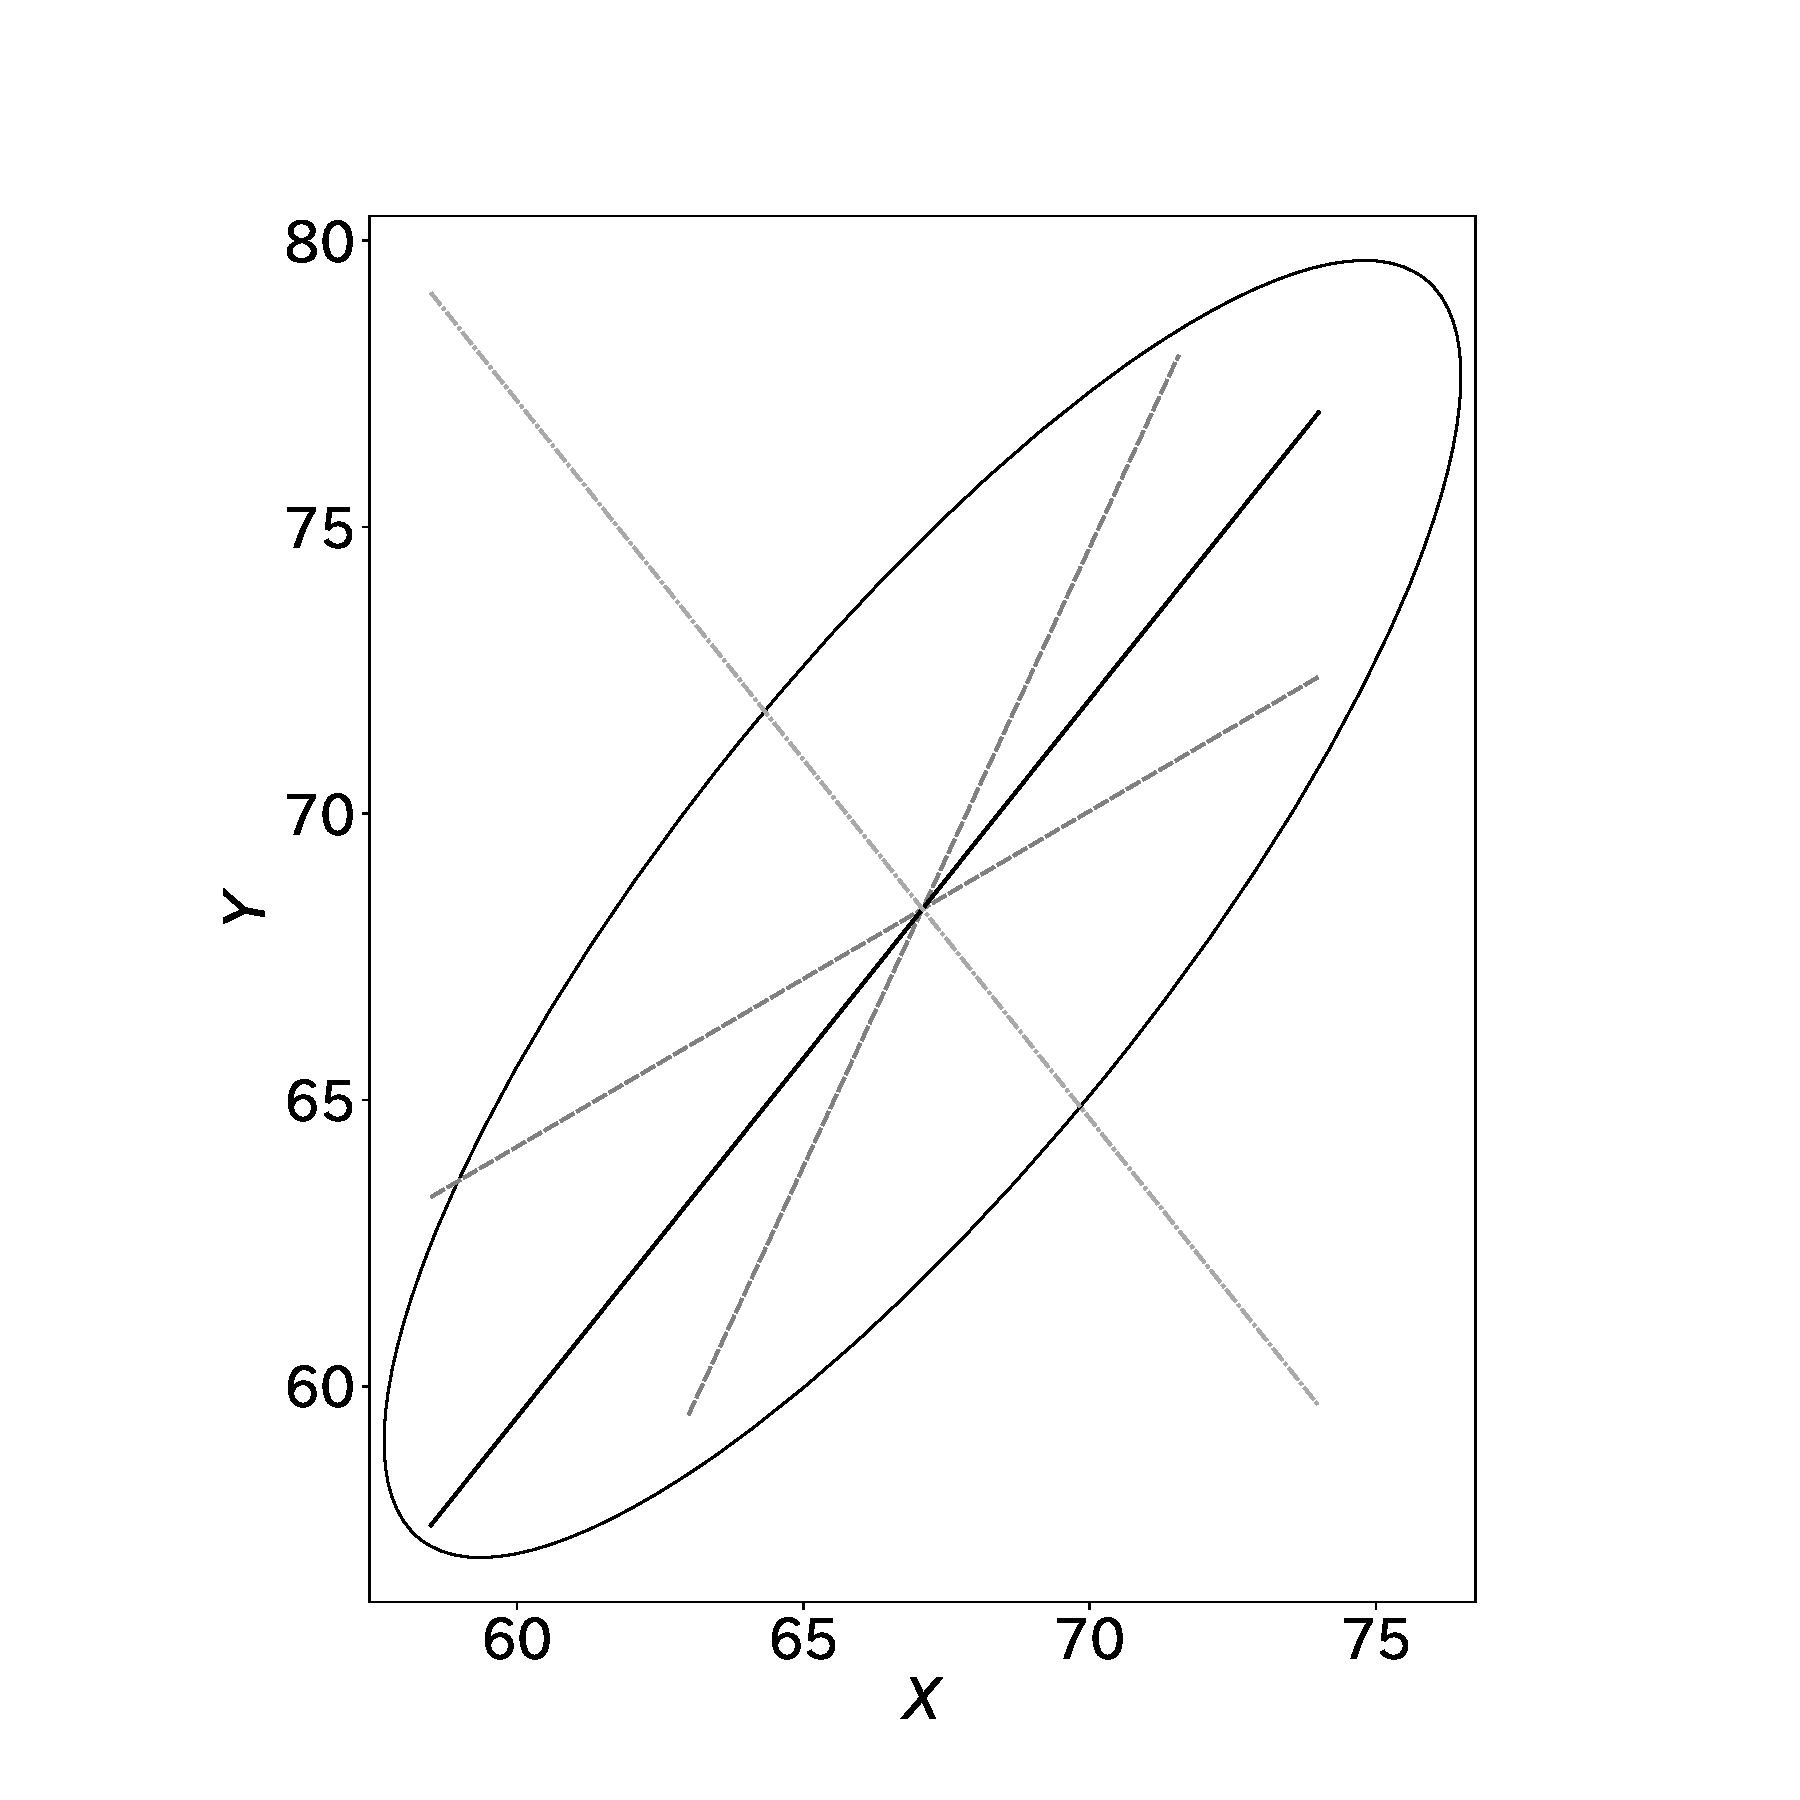
\includegraphics[width=10cm]{./image/16_/multivariate_normal_four_line.pdf}
  \label{fig:multivariate_normal_four_line}
  \caption{二変量モデルにおいて導出される$4$つの直線。傾きが負の直線が短軸であり、それに直行した黒色の直線が長軸である。傾きが正である物のなかで最も小さい傾きをもつ直線が$E[Y|X]$であり、長軸の直線よりも傾きの大きな直線が$E[X|Y]$である。}
 \end{center}
\end{figure}



まず、$Y$を直線$aX+b$により予測するさいの、予測の良さについて考える。
ここでは、評価指標として、$RMSE$を使う。
\begin{eqnarray*}
 \rm{RMSE} &=& \frac{1}{n}\sum_{i=1}^n((y_i-\mu_y)-a(x_i-\mu_x))^2\\
 &=& \frac{1}{n}\sum_{i=1}^n((y_i-\mu_y)^2+a^2(x_i-\mu_x)^2-2a(x_i-\mu_x)(y_i-\mu_y))\\
&=& \frac{1}{n}\sum_{i=1}^n (\sigma_y^2+a^2\sigma_x^2-2a\sigma_{xy})\\
\end{eqnarray*}
これは、$a$に関する二次方程式なので、$\rm{RMSE}$が最小になるのは、$a$が次のときである。
\begin{equation*}
 a = \frac{\sigma_{xy}}{\sigma_x^2}
\end{equation*}
この結果から、$X$をもとに$Y$を予測する直線$E[Y|X]$は、その直線の中では$RMSE$が最小である。
同様に、$Y$をもとに$X$を予測する直線$E[X|Y]$は、その直線の中では$RMSE$が最小である。

\subsection{ちょっと平均によせて}
$E[x_2|x_1]$の傾きは、$\rho\frac{\sigma_x}{\sigma_y}$である。
分散がほぼ等しい状況を考えると、平均からの差分を$\rho$倍して$\mu_2$に足しすことで、$x_2$の予測値となる。$\rho^2$が$1$よりも十分小ければ、予測値は$\mu_2$に近い値となる。言い替えると、$x_1$から$x_2$を予測するには、$x_1$を予測値とするよりも、$\mu_2$に近い値をとることで、分散が小さくなる。



\section{相関係数}
相関係数を次のように定義する。
\begin{equation*}
 \rho = \frac{\sigma_{xy}}{\sqrt{\sigma_x^2\sigma_y^2}}
\end{equation*}
2変量正規モデルににおいて相関係数をBravais-Pearson(ブラベー・ピアソン)の係数と呼ぶこともある。
相関係数$r$の二乗は、実現値が伸びている軸(大きな固有値をもつ固有ベクトル)のまわりにバラついている程度を示す。$r^2$が$1$に近いほど、その軸の上に実現値が乗っており、$0$に近いほど、軸からのばらつき具合が大きくなる。
また、最尤推定量から計算した最尤相関係数は次の様に定義される。
\begin{equation*}
 \rho_{\rm{ML}} = \frac{\sigma_{xy,\rm{ML}}}{\sqrt{\sigma_{x,\rm{ML}}^2\sigma_{y^,\rm{ML}}^2}}
\end{equation*}


具体的に、共分散を設定し、$\rho$に依存した実現値$(x,y)$のばらつきかたを確認する。
図\ref{fig:Correlation_variation_depends_covariance}には、相関係数を設定したとき、モデル
$M(\tra(20,20),\sigma_x^2=\sigma_y^2=2^2,\sigma_{xy})$からサンプリングした実現値がどのようにばらつくのかを示した。
主軸の傾きは、$\sigma_x=\sigma_y$より$1$であり、このとき既に示した様に、主軸の傾きは相関係数$\rho$にはほとんど依存しない。
(A)は相関係数が$0$であり、ほぼ円上(楕円上)に実現値がばらつく。
(B)は相関係数が$0.745$であり、主軸上を中心に楕円上に実現値がばらついていることがわかる。
(C)は相関係数がほぼ$1$であり、主軸上に実現値乗っていることがわかる。
このことから、相関係数は、実現値が主軸上にあつまっている程度を示している。


\begin{figure}
 \begin{center}
  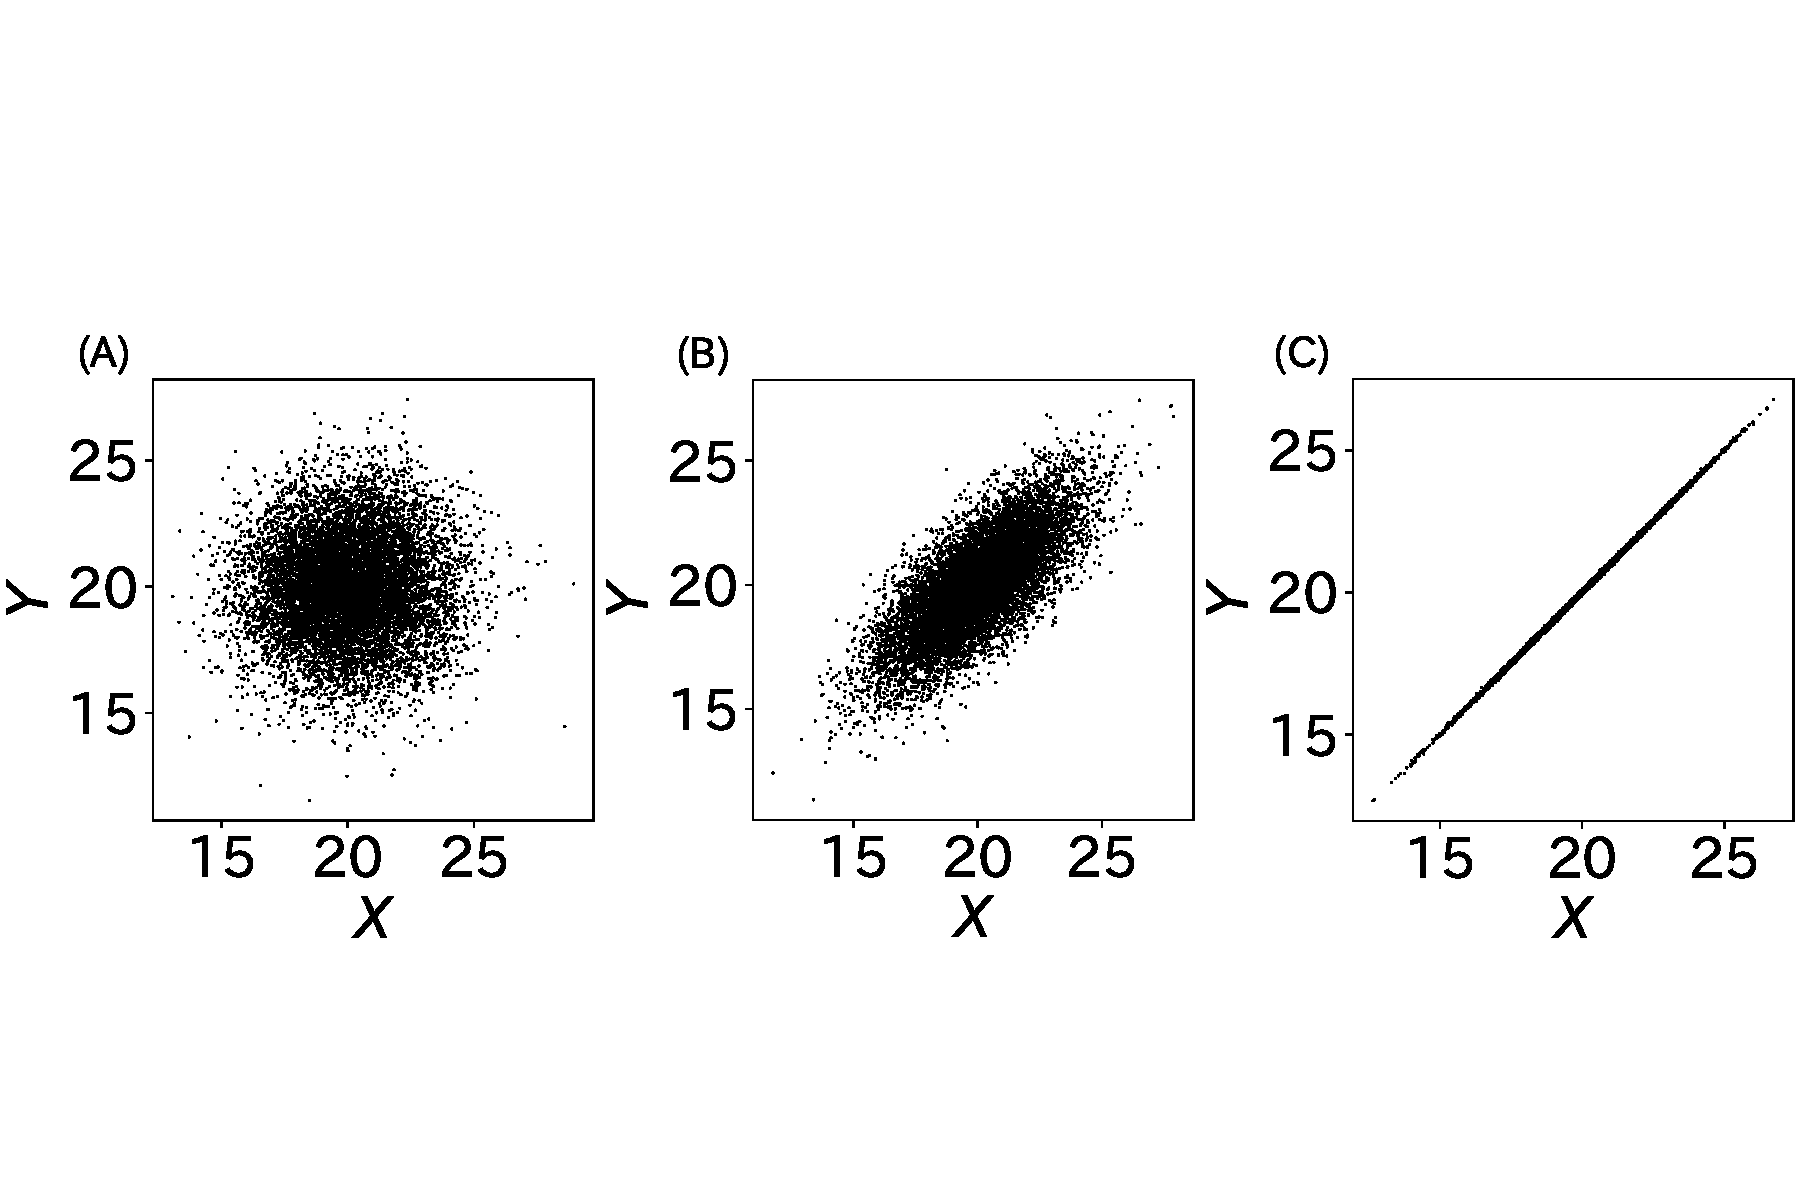
\includegraphics[width=12cm]{./image/16_/Correlation_variation_depends_covariance.pdf}
  \label{fig:Correlation_variation_depends_covariance}
  \caption{実現値のばらつきかた。(a)$\rho= 0.25$(b)$\rho=0.745$(c)$\rho=0.99975$。$\sigma_x=\sigma_y$であるため主軸の傾きは$1$。}
 \end{center}
\end{figure}
\begin{comment}
 $(x-\mu_x)(y-\mu_y)$という量を考えてみる。これは$(\mu_x,\mu_y)$を中心にし、
\begin{enumerate}
 \item $(x,y)$が右上にあれば、$x-\mu_x$と$y-\mu_y$はともに正であり、その積も正
 \item $(x,y)$が左下にあれば、$x-\mu_x$と$y-\mu_y$はともに負であり、その積は正
 \item $(x,y)$が左上にあれば、$x-\mu_x$は負そして、$y-\mu_y$は正であり、その積は負
 \item $(x,y)$が右下にあれば、$x-\mu_x$は正そして、$y-\mu_y$は負であり、その積は負
\end{enumerate}
である。以上から、$(x-\mu_x)(y-\mu_y)$は2次元平面上でのある中心からデータのばらつき方を示す量であること、
そして、その平均は、平均的なデータのばらつきかたを示す。言い替えれば、平均的にデータが$(\mu_x,\mu_y)$を中心に右上から左下に多く存在すれば、共分散は正の値をとることが期待される。
共分散を$\sigma_x,\sigma_y$により規格化した量が相関係数である。

相関係数は、二つの変数が確率変数であることを仮定したモデルにより定義できる量である。

\end{comment}


\subsection{$r^2\leq 1$の証明}
コーシーシュワルツの不等式
$a_1,a_2,\cdots,a_n,b_1,b2,\cdots,b_n$を実数とする。
\begin{equation*}
 (\sum_{i=1}^n a_i b_i)^2 \leq (\sum_{i=1}^n a_i^2)(\sum_{i=1}^n b_i^2)
\end{equation*}
である。等号成立は、$a_i=0$または$b_i=0$または$b_1/a_1=b_2/a_2=\cdots=b_n/a_n$が成り立つときである。

このことを利用する。$a_i=x_i-\bar{x},b_i=y_i-\bar{y}$とおく。
\begin{equation*}
 \left(\sum_{i=1}^n (x_i-\bar{x})(y_i-\bar{y})\right)^2 \leq  \sum_{i=1}^n(x_i-\bar{x})^2\sum_{i=1}^n(y_i-\bar{y})^2
\end{equation*}
このことから、$r^2\leq 1$であり、$-1\leq r \leq 1$がわかる。


%



\begin{SMbox}{相関係数}
 次のような記述を見たことがあるだろう\footnote{Google検索で「相関係数 論文 書き方」などで調べれば見付けられる。ただし、この全てが本書の方針と異るかは不明。}。
\begin{quote}
 有意な相関係数が得られた($r=0.2(p<0.05,n=10)$)。
\end{quote}
これは、二つのモデルに関して述べられている。1つは共分散が$0$の二変量正規モデルとデータがかいりしているということである。これが$p<0.05$で表現されている。もう一つは、最尤二変量正規モデルにおいて、相関係数が$r=0.2$であったことである。
 これらを同時に表現すると、「有意な(あるモデルでは予測できない)相関係数(最尤推定モデルから得られる要約量)が得られた」となる。
 
 これら二つは別のモデルの事なので、「有意だから、相関係数に意味がある」や「有意ではないから、相関係数に意味がある」についてはどちらも言えない。
 ただし、論文統計学では、最尤モデルの相関係数に意味があることをヌルモデルによる有意性により論じることができるということになっている。
 これは、$p<0.05$であれば、どんなに小さな$r$でも意味があることになってしまう。
 後で述べるが、$r=0.1$である場合、平均値による予測により得られる誤差を$1\%$しか改善していない。

 $1\%$の精度改善に意味があるのかは研究対象に依存するだろう。
 例えば、様々な要素を調査したとしても、平均値モデルよりも精度改善しなかったが、ある特定の量で$1\%$の精度改善がみられたならば、その発見は意味があるかもしれない。
 %後で述べるが、$r=0.2$である場合、平均値による予測により得られる誤差を$4\%$しか改善していない。これが意味があるのかを検定で調べることは本書では推奨しない。
\end{SMbox}

\subsection{決定係数$R^2$と相関係数$\rho^2$の関係}
$E[x_2|x_2]$による予測において、決定係数$R^2$と相関係数$\rho^2$の関係を調べる。
これを用いて、残差平方和の計算をおこなう。
\begin{eqnarray*}
 \sum_{i=1}^n (y_i-E[x_2|x_i])^2 &=&   \sum_{i=1}^n ((y_i-\bar{y})^2+\frac{\sigma^2_{xy}}{\sigma^4_x}(x_i-\bar{x})^2-2\frac{\sigma_{xy}}{\sigma^2_x}(x_1-\mu_1)(x_2-\mu_2))\\
 &=& n\sigma^2_y -n \frac{\sigma^2_{xy}}{\sigma_x^2} \\
 &=& n\sigma_y^2(1-\frac{\sigma^2_{xy}}{\sigma^2_x\sigma_y^2}) \\
 &=& n\sigma_y^2(1-\rho^2)
\end{eqnarray*}
以上より、平均二乗誤差は、以下とも等しい。
%ここで、回帰平均二乗誤差RMSE(regression mean square)を定義しておく。
\begin{equation*}
 %RMSE^2 = 
 RSS^2 = (\sigma_y\sqrt{1-\rho^2})^2
\end{equation*}
このことを用いて、決定係数$R^2$について計算を行う。
\begin{eqnarray*}
 R^2 &=& 1-\frac{\sum_{i=1}^n e_i^2}{\sum_{i=1}^n (y_i-\bar{y})^2} \\
 &=& 1-\frac{n\sigma_y^2(1-\rho^2)}{n\sigma^2_y} \\
 &=& \left( \frac{\sigma_{xy}}{\sigma_x\sigma_y}\right)^2 = \rho^2
\end{eqnarray*}

%誤差モデルにおいては、
このことから$x_2$の$x_1$に対する回帰においては、決定係数と相関係数の二乗が一致することがわかる。
また、$0\leq R^2\leq 1$であることもわかる\footnote{直感的に、平均よりも悪くなることはないので、$0\leq R^2$も明らか}。
%このように計算をおこなわなくても、誤差モデルにおいて$0\leq R^2\leq 1$が成立することは、平均値よりも予測がわるくなることはなさそうであるので、$0\leq R^2$は明らか。

\paragraph{決定係数の意味}
決定係数は、平均値による予測と比べて、提案した誤差モデルでの予測がどれくらい良くなったのかを示す指標である。
第二項は、分母に、平均と観測値の差の二乗、分子に予測値と観測値の差の二乗をしたものである。
予測性能が良ければ、分子が小くなり、第二項が$0$に近くなり、決定係数は$1$に近付く。
予測性能がわるければ、分子が大きくなり、平均よりも悪い予測をおこなうならば、決定係数は負になる。

\subsection{相関係数が$0.8$のとき}
相関係数が$0.8$のとき、$RMSE$は、$RMSE^2 = \sigma_y\sqrt{1-\rho^2}$より、
\begin{equation*}
 RMSE = 0.6\sigma
\end{equation*}
である。
これは、回帰により二乗誤差が$\sigma$からその$0.6$倍改善されたことを示している。
また、確率変数による予測は$\sqrt{2}\sigma$なので、このモデルと比較すると、
\begin{equation*}
 0.6\sigma = 0.428(\sqrt{2})\sigma
\end{equation*}
より、$0.42倍$改善されている\footnote{https://mathlog.info/articles/2936}
ランダムヌルモデルの$RMSE$の$58\%$割引ともいえる。

また、$R^2$が相関係数と一致することから、次が成り立つ。
\begin{equation*}
 \frac{線形モデルと観測値の二乗誤差}{平均と観測値の二乗誤差} = 1-0.64 = 0.36
\end{equation*}
このことから、
\begin{equation*}
 線形モデルと観測値の二乗誤差 = 0.36平均と観測値の二乗誤差
\end{equation*}
平均と観測値の二乗誤差の$64\%$引きが線形モデルと観測値の二乗誤差である。
同様に、相関係数が$0.2$だとすると、平均と観測値の二乗誤差の$4\%$引きが線形モデルと観測値の二乗誤差である。
相関係数を予測性能を示す統計量とあわせて考えると、相関係数が$0.2$だとたったの$4\%$しか性能が改善されていないことがわかる。
平均値による誤差の半額引きには、相関係数$0.7$程度が必要である。

\begin{SMbox}{$4\%$の改善}
 $4\%$の改善がみられたことは報告するべきことだろうか。それは、業界や対象に依存する。さまざまな、要素との対応関係を調べたが$1\%$も性能が改善されない対象であれば、$4\%$の性能改善はすごい発見であろう。また、ある要素との対応関係で$96\%$程度改善されているような対象であれば、$4\%$の改善を発見するというのは小さな発見とも思える。

 %ただし、あらゆる実験報告には価値がある。
\end{SMbox}


\subsection{ヌルモデルの相関係数}
2変量正規モデルその共分散が$0$のモデルにおいて、相関係数を含む次の$T$が自由度$n-2$の$t$分布に従う\footnote{正規2モデル$M(\mu_x,\mu_y,\sigma_x^2,\sigma_y^2)$において$T$がある分布に従うと言ってもいいが、相関係数を計算するとき、我々の頭のなかには2変量正規モデルでみてみようという考えがあり、正規モデルは頭にないはずである。}\footnote{$r$が従う分布も計算できるようである。Wikipediaに記述があるが、これが正しいことを私は確かめていない。\url{https://en.wikipedia.org/wiki/Pearson_correlation_coefficient#Using_the_exact_distribution}}。
言い替えれば、モデル$M(\mu,\sigma_x,\sigma_y,\sigma_{xy}=0)$からサンプリングした標本から、その最尤モデルを構築し、その相関係数から以下の$T$を計算する。
この作業を繰り返すと、$t_{n-2}$に従うということがわかる。
\begin{equation*}
 T = r\frac{\sqrt{n-2}}{\sqrt{1-r^2}} \sim t_{n-2}
\end{equation*}
ここで、$n$はサンプルサイズ、$t_{n-2}$は、自由度$n-2$の$t$分布。
このことを利用して、データと2変量正規モデル間の乖離具合を調べることができる。
%これは、相関係数に対する検定と呼ばれる作業に対応する。
\subsubsection{数値計算}
二変量正規モデル$M(\vecc{\mu}=\tra (0,0),\sigma_x=2,\sigma_y=1,\sigma_{xy}=0)$とする。
このモデルからサンプルサイズ$10^4$の標本を$10^4$個を作成し、標本の個数分、相関係数また$T$値を計算した。
結果は図\ref{fig:Correlation_null_model}に示した。数値実験の累積分布が$t$分布の累積分布と一致した。

\begin{lstlisting}
sigma = np.array([[2**2,0],[0,1**2]])
mu=np.array([10,20])
sampleN = 10**4
N= 10**4
sample = multivariate_normal(mu,sigma).rvs(size=(sampleN,N))

mu = np.mean(sample,axis=1)
cov = np.array([np.cov((sample[idx]-mu[idx]).T) for idx in range(sampleN)])
r = np.array([cov[idx][0,1]/np.sqrt(cov[idx][0,0]*cov[idx][1,1]) for idx in range(sampleN)])
T = r*np.sqrt(N-2)/np.sqrt(1-r**2)
\end{lstlisting}


\begin{figure}
 \begin{center}
  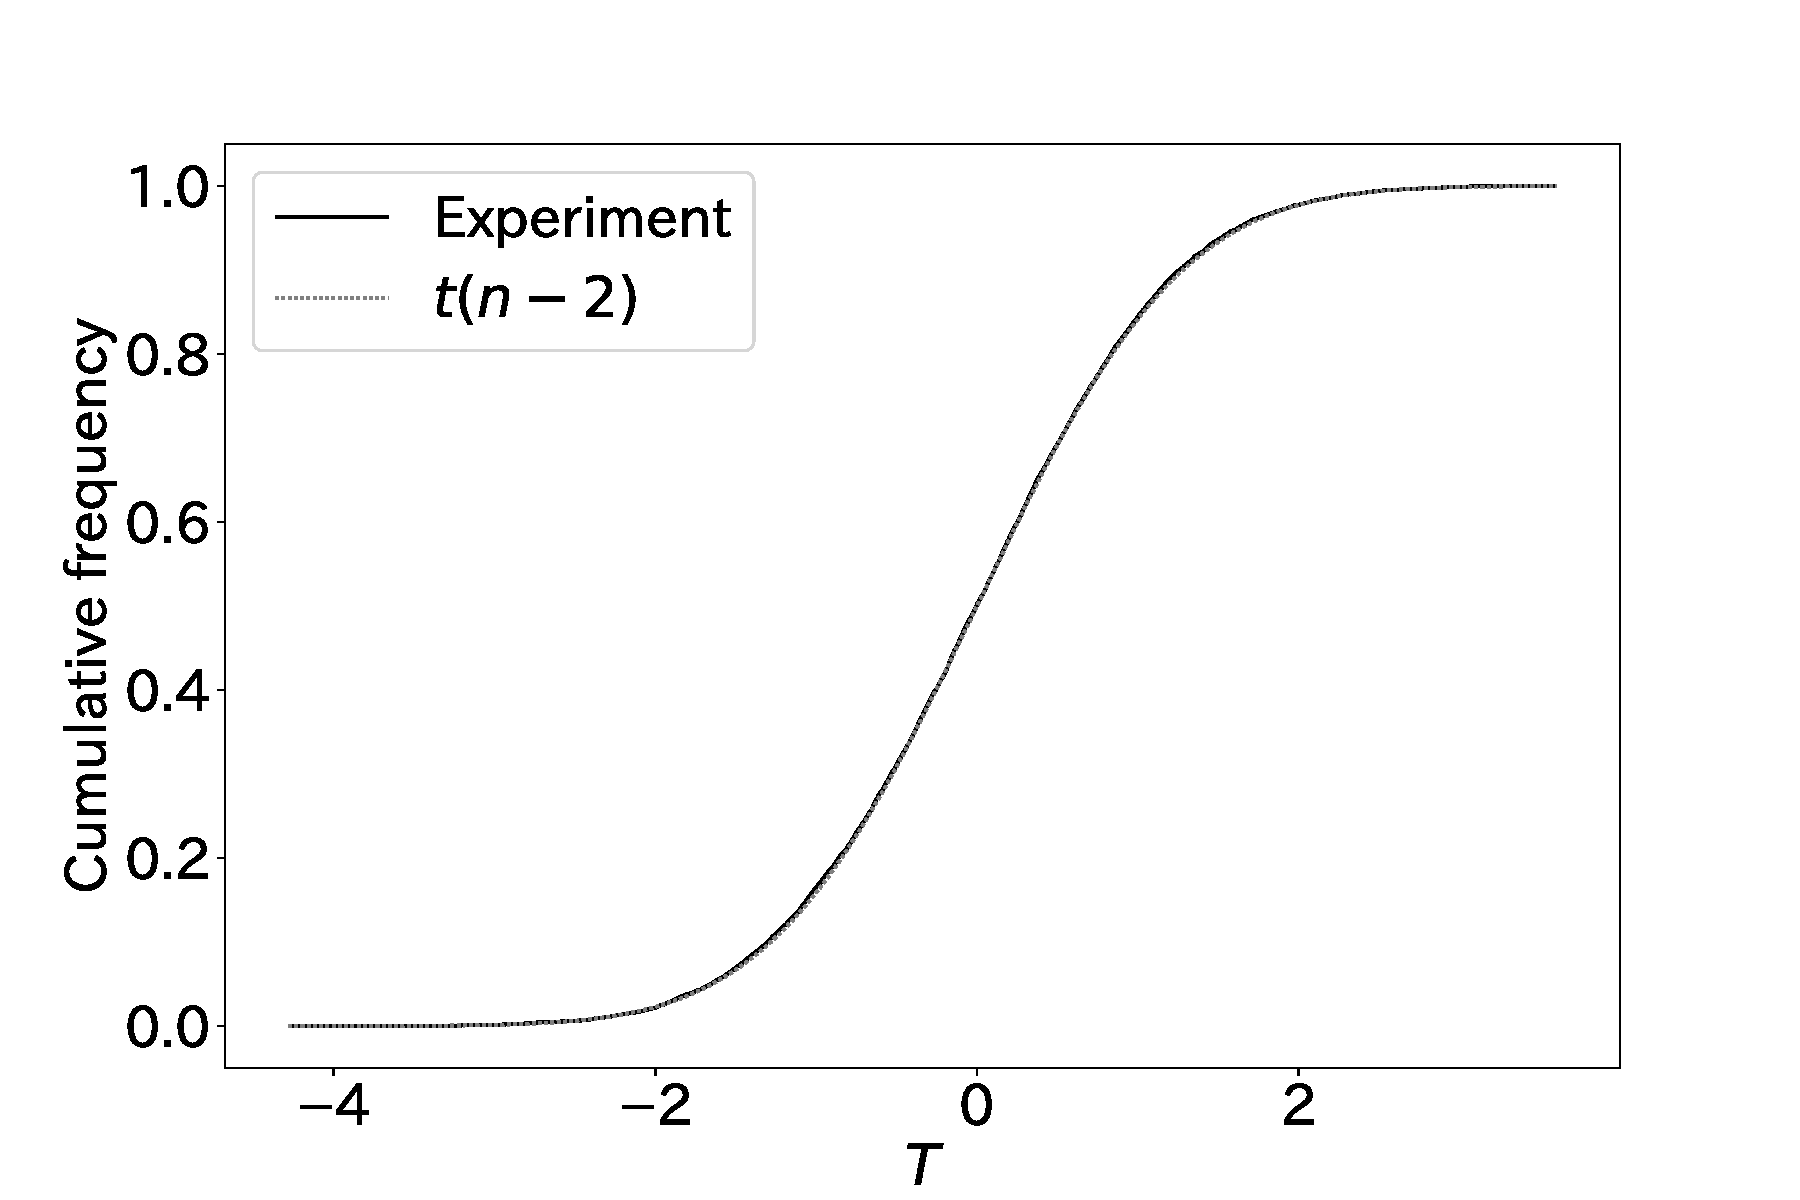
\includegraphics[width=15cm]{./image/16_/Correlation_null_model.pdf}
  \label{fig:Correlation_null_model}
  \caption{$T$値の累積分布}
 \end{center}
\end{figure}







\section{軸と重なる直線}
二変量モデルの共分散係数の1つ$\sigma_x^2$は、このモデルにおいてバラツキかたを示していないことがある。例えば、共分散行列$\sigma_x^2=2,\sigma_y^2=1,\sigma_{xy}=0$とする。
このとき、確率変数は平均を中心に$x$軸方向でのバラツキが大きく、また楕円形に広がる。

\begin{figure}
 \begin{center}
  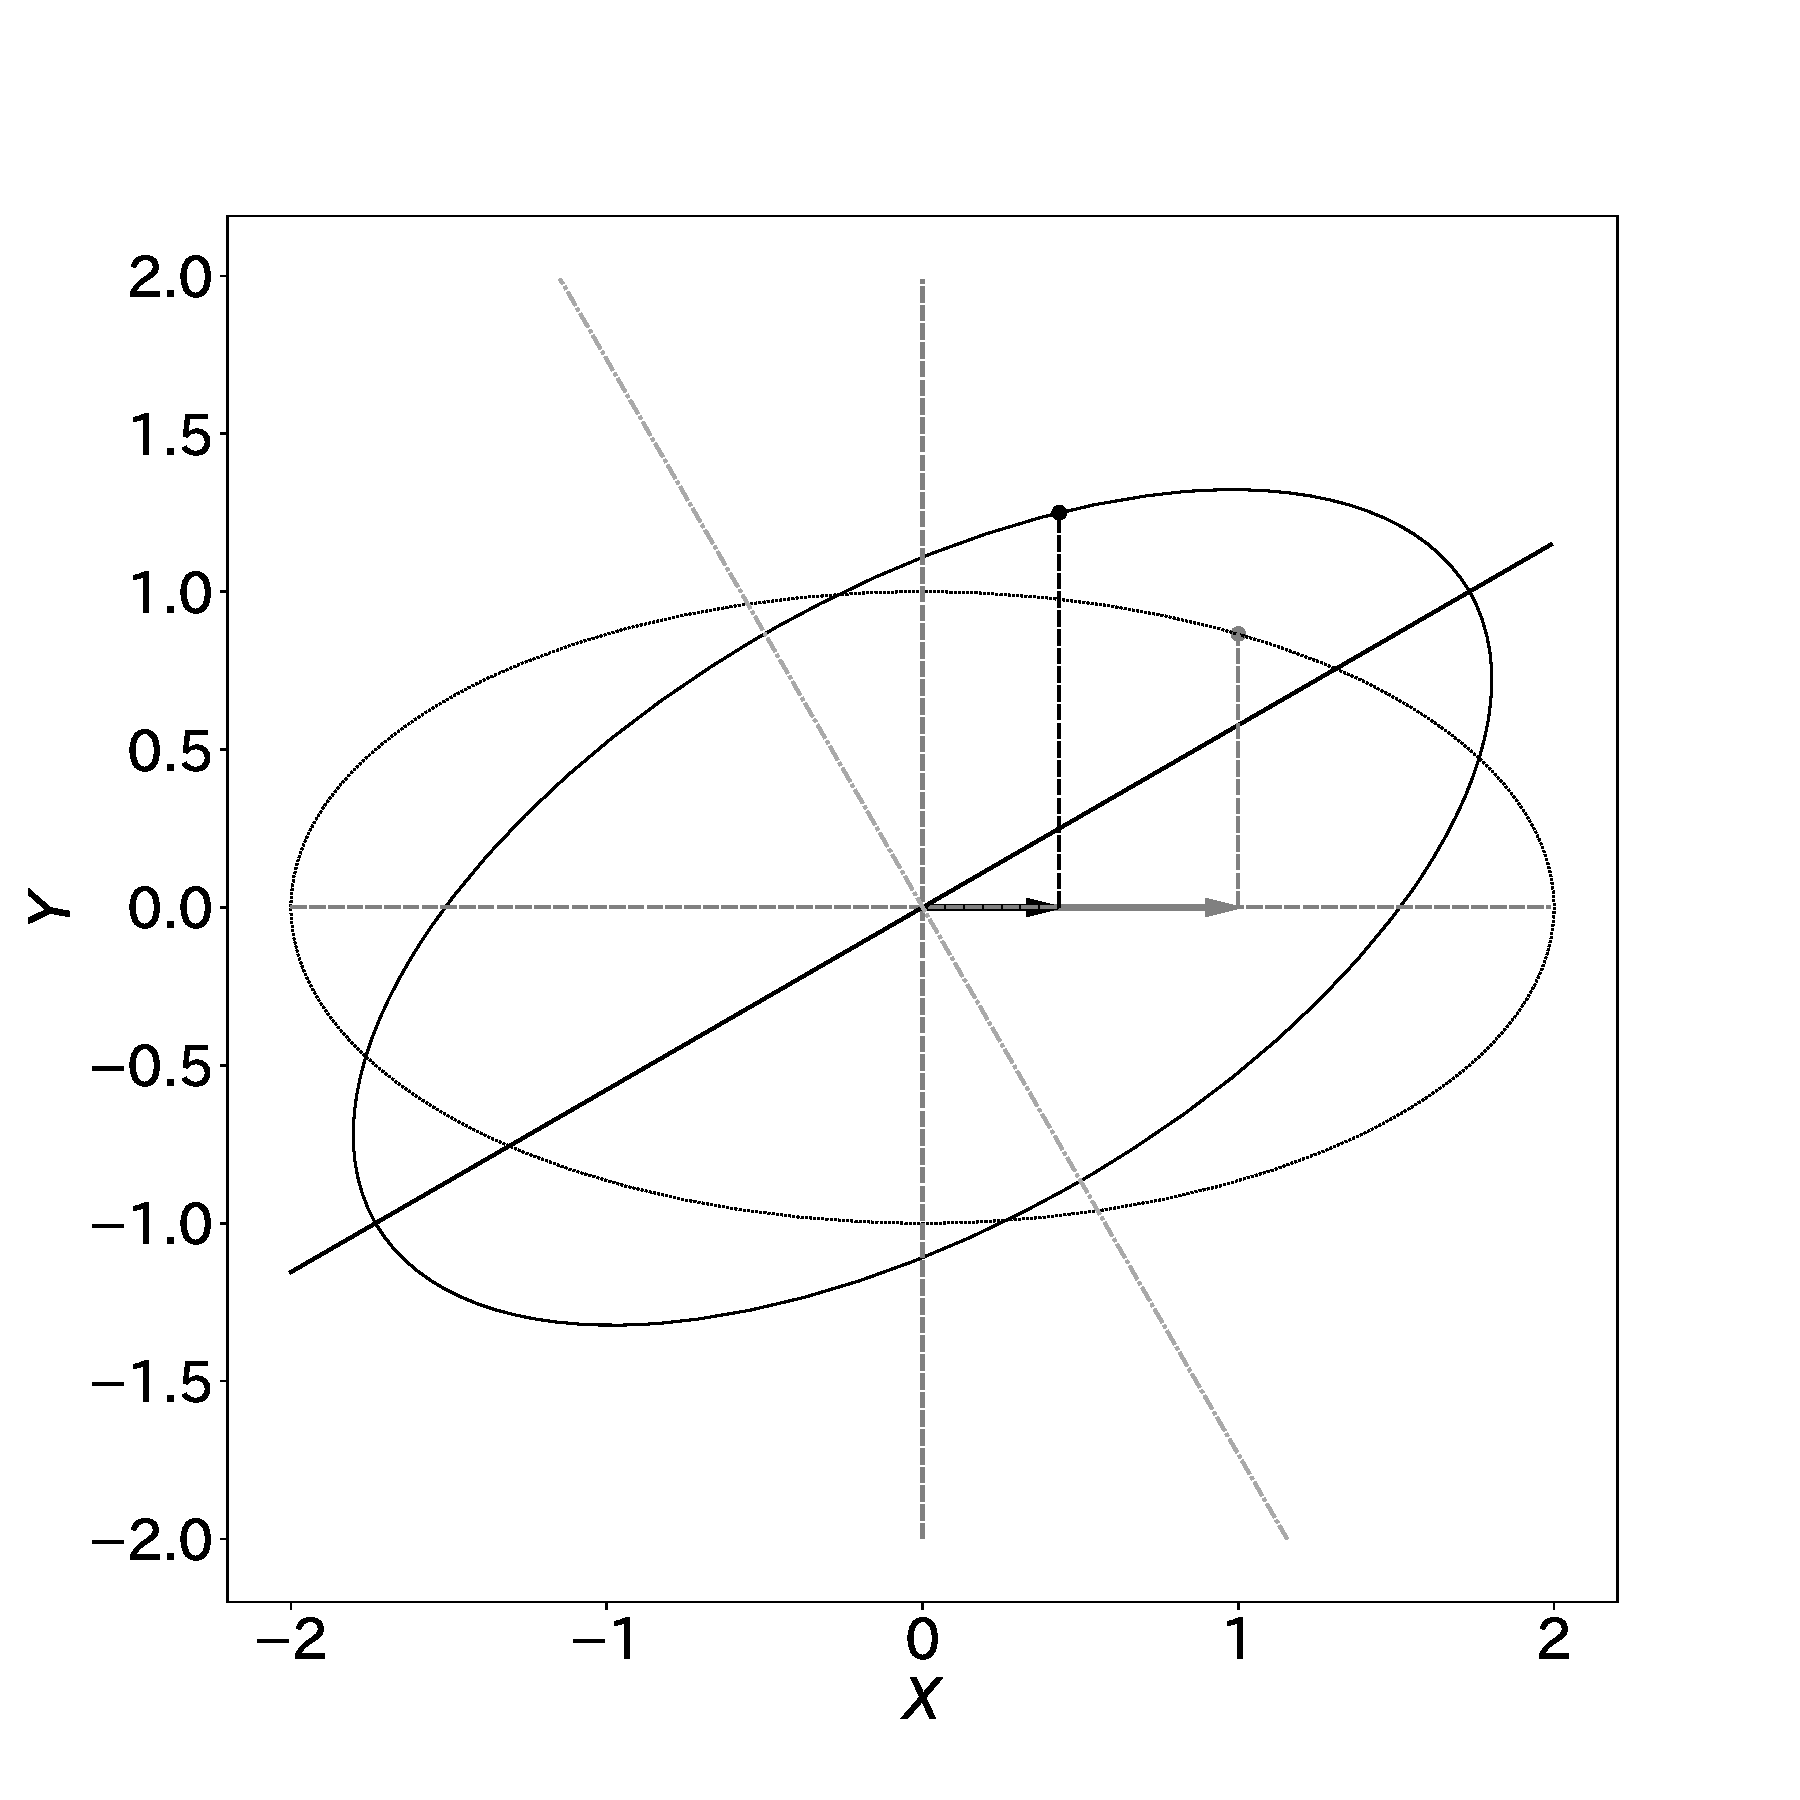
\includegraphics[width=10cm]{./image/16_/ellipse_x_axis_twice_angle_pi_6.pdf}
  \label{fig:ellipse_x_axis_twice_angle_pi_6}
  \caption{回転していない楕円(破線)と$\pi/6$回転した楕円(実線)。灰色の点は回転していない楕円上の点、黒色の点は$\pi/6$だけ原点を中心に灰色の点を回転させた点。}
 \end{center}
\end{figure}

共分散が$0$より大きくなると、楕円が回転する。図\ref{fig:ellipse_x_axis_twice_angle_pi_6}はこの楕円の回転の様子を描画した。
回転していない楕円上の点(灰色)を$\pi/6$回転した点を黒く描画している。
灰色の点の$x$軸方向の分散は、灰色の矢印間の距離の二乗を平均したものであった。
さまざまな確率変数を集め、矢印間の距離の二乗を平均を計算したものが、$\sigma_x^2=2$であった。
同様の操作を$\pi/6$回転した楕円でおこなうと$\sigma_x^2$が得られるだろうか?
黒色の点を$x$軸に射影した点と原点との距離を黒色の矢印でしめした。
黒色の矢印は灰色の矢印と比べると小くなっている。
これを回転させた楕円のなかでばらつく確率変数について計算すると、分散が小くなっている。
単に$X$のばらつきを計算しただけでは、ばらつき方に関する量として不十分であることを示している。
このことは、回転させた楕円のなかで散らばる確率変数については、ばらつきを工夫して計算する必要があることを示唆している。

\begin{figure}
 \begin{center}
  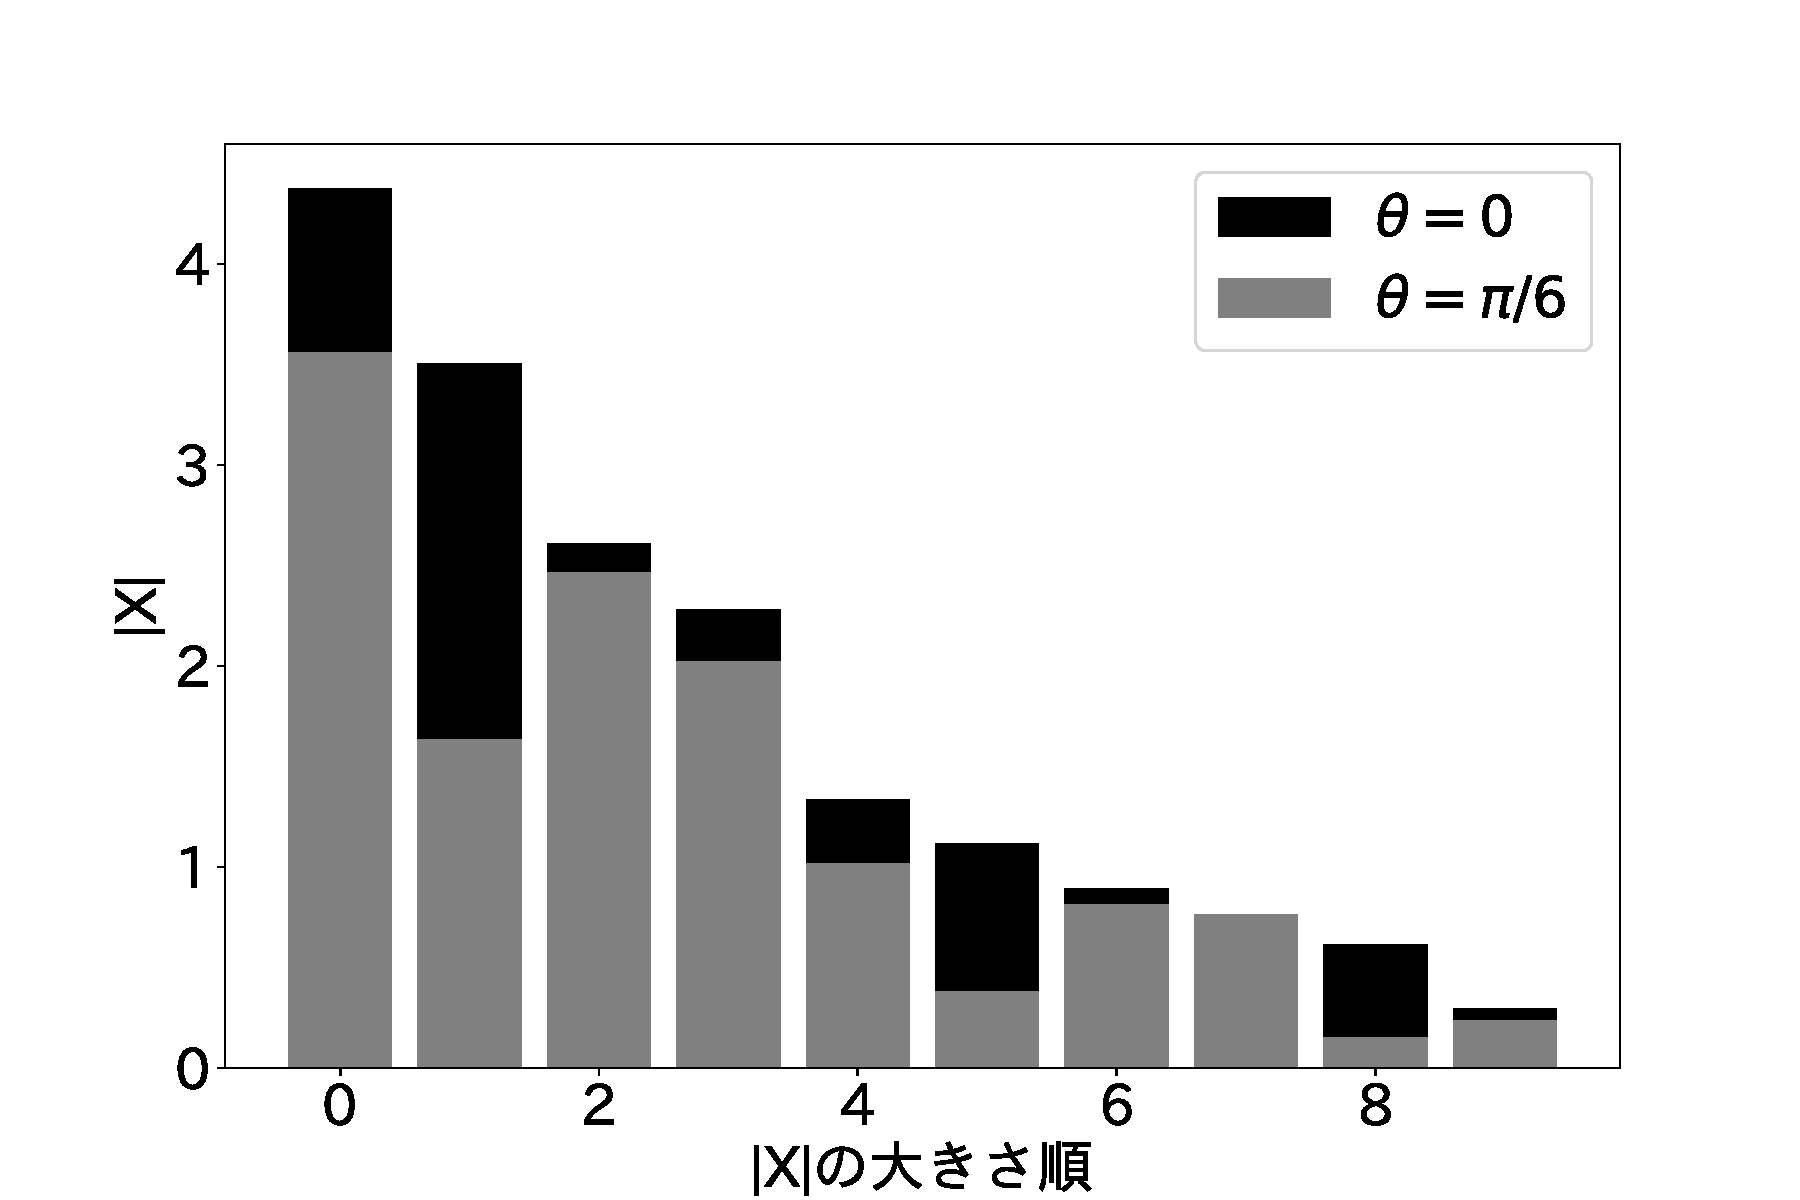
\includegraphics[width=10cm]{./image/16_/ellipse_distributed_X_comparison.pdf}
  \label{fig:ellipse_distributed_X_comparison}
  \caption{回転していない楕円に従い広がるように生成した乱数の$|X|$の大きさ(黒)と、座標を$\pi/6$回転させた座標での$|X|$(灰色)。回転させた座標の$|X|$のほうが回転前の$|X|$よりも小くなっている。}
 \end{center}
\end{figure}


そこで、単に$x$軸に射影したときのばらつきではなく、ばらつきがもっとも大きくなる軸を計算する方法を考える。
ある直行する2つのベクトルに対し、そのベクトルが貼る空間を$U-V$空間と言う。これは、回転させたときの座標空間のことである。
ここで、その基底ベクトルを$\vecc{e_u}=\tra (u_1,v_1),\vecc{e_v}=\tra (u_2,v_2)$と表記する。$X-Y$空間上の点$(x,y)$を$U-V$空間のベクトルで表すには、ベクトル$\vecc{k}=\tra(k_1,k_2)$を用いて、
\begin{equation*}
 \vecc{x} = P\vecc{k} = \begin{pmatrix}
u_1 & u_2 \\
v_1 & v_2 \\
\end{pmatrix}\vecc{k}
\end{equation*}
転置を行った表記では、$\tra x = \tra k \tra P$である。
また、$X-Y$座標から、$U-V$空間への変換は$(k_1,k_2)=(x,y)P$と表記できる。

\begin{figure}
 \begin{center}
  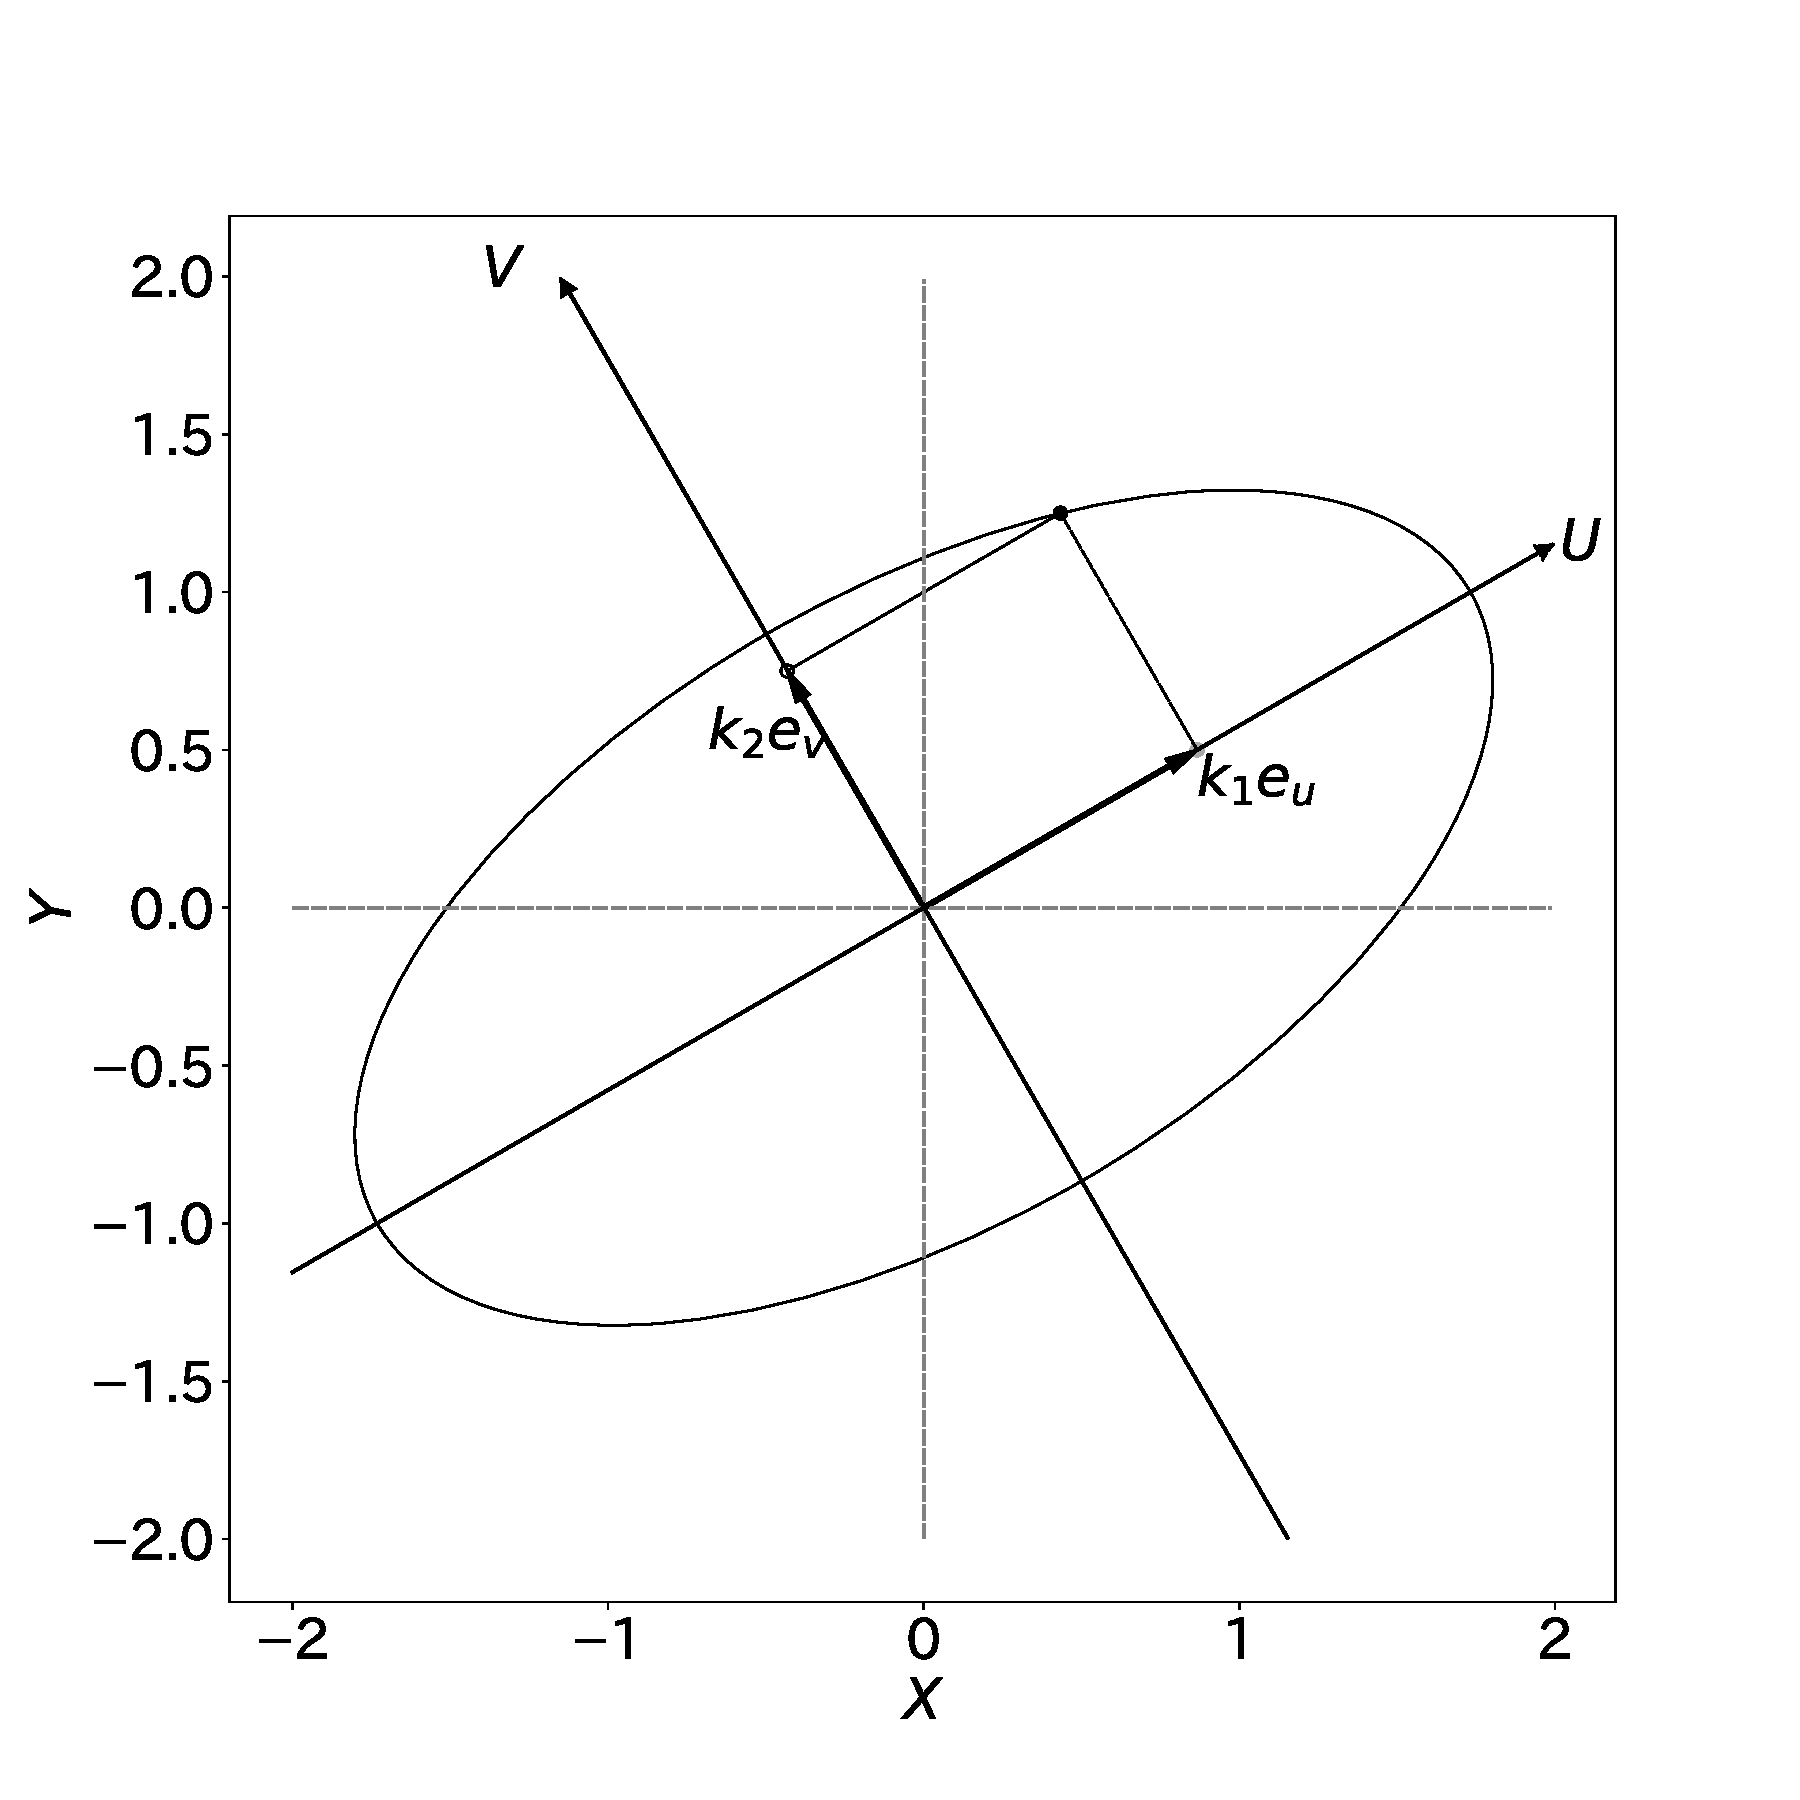
\includegraphics[width=10cm]{./image/16_/ellipse_U_V_plane.pdf}
  \label{fig:ellipse_U_V_plane}
  \caption{$U-V$平面上での座標点の表現。黒色の点$\vecc{x}$を単位ベクトル$\vecc{e_u},\vecc{e_v}$により表現するには、ベクトル$(k_1,k_2)$を用いることで実現できる。$\vecc{x}=k_1\vecc{e_u}+k_2\vecc{e_v}=P\vecc{k}$である。}
 \end{center}
\end{figure}

楕円状に広がったデータを並べた$n\times 2$行列を$A$とする。
\begin{equation*}
 A =\begin{pmatrix}
     x_1 & y_1 \\
     x_2 & y_2 \\
     \vdots & \vdots \\
     x_n & y_n \\
 \end{pmatrix}
\end{equation*}
$X-Y$空間での共分散行列は、$\tra A A$により計算できる。
この行列$A$を$U-V$空間上で表すには、$A$に$P$を左から作用させればよい。これを$K=AP$とする。
$U-V$空間上での共分散行列は、$\tra KK$を計算すれば求められる。
\begin{equation*}
 \tra KK = \tra (AP)(AP) = \tra P\Sigma P
\end{equation*}
この式において$\vecc{e_u}$が係る部分は、$\tra\vecc{e_u} \Sigma \vecc{e_u}$である。
ラグランジュの未定乗数法を用いることで、$\tra\vecc{e_u} \Sigma \vecc{e_u}$を最大かつ$|\vecc{e_u}|=1$となる$\vecc{e_u}$を求めることができる。
具体的には、
\begin{eqnarray*}
 F(\vecc{e_u}) = \tra\vecc{e_u} \Sigma \vecc{e_u}-\lambda(|\vecc{e_u}|-1)
\end{eqnarray*}
が最大となる点を求める。$\frac{\partial}{\partial \vecc{e_u}}F = \frac{\partial }{\partial \lambda}F = 0$となる$\vecc{e_u}$をさがす。
\begin{eqnarray*}
 \frac{\partial}{\partial \vecc{e_u}}F = 2\Sigma \vecc{e_u}-2\lambda \vecc{e_u} = 0
\end{eqnarray*}
これを満す$\vecc{e_u}$を求めればよい。整理すると次が得られる。
\begin{equation*}
 \Sigma \vecc{e_u} = \lambda \vecc{e_u}
\end{equation*}
これは明かに、$\Sigma$に対する固有値問題である。
同様に、$\vecc{e_v}$についても$\Sigma$に関する固有値の計算を行えばよい。


以上のことから、$U-V$空間上の共分散行列$\tra KK$が最大になる$\vecc{e_u},\vecc{e_v}$と固有値問題が対応付けられる。
また、固有値はデータの固有ベクトル上でのばらつき方をしめしており、固有ベクトルはばらつきが最大になるようなベクトルである。また、固有値は、固有ベクトル空間上においてデータのばらつきかたを示している。
この固有ベクトルの方向と一致する直線が主軸直線であり、この直線のまわりに実現値がばらつく。

\section{マハラノビス距離}
モデルの2つの実現値$\vecc{x},\vecc{y}\in \mathbb{R}^2$の間の距離$d$を次の様に定める。
\begin{equation*}
 d(\vecc{x},\vecc{y}) = \sqrt{\tra(\vecc{x}-\vecc{y})\Sigma^{-1} (\vecc{x}-\vecc{y})}
\end{equation*}
ここで、$\Sigma$は共分散行列である。

また、2変量正規モデルにおける中心座標を$\vecc{\mu}$とし、中心とある実現値$\vecc{x}$の間の距離$D$を次の様に定める。
\begin{equation*}
 D_M(\vec{x}) = d(\vecc{x},\vecc{\mu})
\end{equation*}
この距離は、既に見たように2変量正規分布の確率密度関数の指数部分と一致していることから、楕円の式となることがわかる。

この距離$D_M$は$D_M(\vecc{x})^2\sim \chi^2_2$であることが知られている。
このことから、$D_M(\vecc{x})^2 = \chi^2_2(0.68)=2.27$となる楕円の内側に実現値のおおよそ$68\%$が含まれている。

\subsubsection{数値計算}
数値計算により検証した。
\begin{lstlisting}
sigma = np.array([[2**2,2.99],[2.99,2**2]])
sample1 = multivariate_normal(mu,sigma).rvs(size=(10**5))
def Mahalanobis_distance(sample_,mu_,sigma):
    return np.sqrt(np.sum(((sample_-mu_)@np.linalg.inv(sigma))*(sample_-mu_),axis=1))
D2 = Mahalanobis_distance(sample1,mu,sigma)**2
np.sum(D2<chi2.ppf(0.68,df=2))/len(D2),np.sum(D2<chi2.ppf(0.95,df=2))/len(D2)

Output: (0.68224, 0.95114)
\end{lstlisting}



\if 0
\section{Model I}
\begin{comment}
これはちがう
 with pm.Model() as model1:  # model specifications in PyMC are wrapped in a with-statement
    # Define priors
    xdata = pm.ConstantData("x", x, dims="obs_id")

    sigma = pm.HalfCauchy("sigma", beta=20)
    #sigma = pm.Uniform("sigma",lower=10**-3,upper=10**3)

    intercept = pm.Normal("intercept", 0, sigma=100)
    #intercept = pm.Beta("intercept",alpha=5,beta=1)
    slope = pm.Normal("slope", 0, sigma=100)
    #intercept = pm.Uniform("intercept",lower=10**-3,upper=10**3)

    #slope = pm.Uniform("slope",lower=10**-3,upper=10**3)

    # Define likelihood
    #likelihood = pm.Normal("y", mu=intercept + slope * xdata, sigma=np.sqrt(slope)*sigma, observed=y)
    #likelihood = pm.Normal("y", mu=intercept + slope * xdata, sigma=sigma/np.sqrt(1+slope**2), observed=y)
    likelihood = pm.Normal("y", mu=(intercept + slope * xdata), sigma=sigma, observed=y)
    # Inference!
    # draw 3000 posterior samples using NUTS sampling
    idata = pm.sample(3000,cores=3)
\end{comment}
\fi

\if 0
\section{Model I'}
実数のペア$(x_1,y_1),(x_2,y_2),\cdots,(x_n,y_n)$が次の線形な関係を持つとする。
\begin{comment}
\begin{equation*}
 u_i =x_i -\frac{y_i-a}{b} \ \ (i=1,2,\cdots,n)
\end{equation*} 
\end{comment}
ここで、誤差項が確率変数であることを仮定してモデルModel I'を構築する。
\begin{enumerate}
 \item $x_i$は、与えられた定数
 \item $a,b$を実数の定数
 \item $u_i = x_i -\frac{y_i-b}{a}$
 \item $u_i \sim N(0,\sigma^2)$
 %\item $E[u_i]=0$。平均は$0$。
 %\item $E[u_j u_i]=0$。無相関。
 %\item $Var[u_i]=0$。分散が均一。
\end{enumerate}
この仮定により構築されるモデルを$M_{I'}(a,b; x)$または$M_{I'}(a,b)$と表記する

\subsection{尤度}
このモデルの対数尤度のうち、
\fi
\begin{comment}
 with pm.Model() as model1:  # model specifications in PyMC are wrapped in a with-statement
    # Define priors
    ydata = pm.ConstantData("y", y, dims="obs_id")

    sigma = pm.HalfCauchy("sigma", beta=10)
    #sigma = pm.Uniform("sigma",lower=10**-3,upper=10**3)

    intercept = pm.Normal("intercept", 0, sigma=100)
    #intercept = pm.Beta("intercept",alpha=5,beta=1)
    slope = pm.Normal("slope", 0, sigma=100)
    #intercept = pm.Uniform("intercept",lower=10**-3,upper=10**3)

    #slope = pm.Uniform("slope",lower=10**-3,upper=10**3)

    # Define likelihood
    likelihood = pm.Normal("x", mu=(ydata-intercept)/slope, sigma=sigma, observed=x)

    # Inference!
    idata = pm.sample(3000,cores=3)
\end{comment}

\if 0
\section{Model II'}

\begin{enumerate}
 \item $x_i-u_i \sim N(0,\sigma^2)$
 \item $y_i-v_i \sim N(0,\sigma^2)$
 \item $a,b$を実数の定数
 \item $v_i -a u_i -b = 0$
\end{enumerate}
この仮定により構築されるモデルを$M_{II'}(a,b; x)$または$M_{II'}(a,b)$と表記する

\subsection{最尤モデル}
このモデルの尤度を計算する。
\begin{eqnarray*}
 L &=& \prod_{i=1}^{n}\frac{1}{\sqrt{2\pi\sigma^2}}\exp\left(-\frac{(x_i-u_i)^2}{2\sigma^2} \right)\prod_{i=1}^{n}\frac{1}{\sqrt{2\pi\sigma^2}}\exp\left(-\frac{(y_i-v_i)^2}{2\sigma^2} \right)\\
 &=& \prod_{i=1}^{n}\frac{1}{\sqrt{2\pi\sigma^2}}\exp\left(-\frac{(x_i-u_i)^2+(y_i-v_i)^2}{2\sigma^2} \right)
\end{eqnarray*}
対数尤度で、

\subsection{モデルの拡張}
このモデルは、次の様に、誤差の分散について拡張できる。
\begin{enumerate}
 \item $x_i-u_i \sim N(0,\sigma_x^2)$
 \item $y_i-v_i \sim N(0,\sigma_y^2)$
 \item $a,b$を実数の定数
 \item $v_i -a u_i -b = 0$
\end{enumerate}
このモデルの最尤推定量は、上記と同様のはずなので、詳しくは計算を行わない。
\begin{eqnarray*}
 \hat{a} &=& \frac{Q^2_{yy}-\lambda Q^2_{xx}+\sqrt{(Q^2_{yy}-\lambda Q^2_{xx})^2+4\lambda Q_{xy}}}{2Q_{xy}} \\
 \hat{b} &=& \bar{y}-\hat{a}\bar{x}
\end{eqnarray*}
ここで、$\lambda = \frac{\sigma_x^2}{\sigma_y^2}$である。


\fi




\begin{comment}
 \begin{table}
 \begin{tabular}{llll}
  名前 & 最小化要素 & 最小化関数 & \\
  \hline \hline\\
  Model I regression & && \\

  Regression &$y$軸方向の変動を最小化 & $s_{y,x}(\Delta y^2)$ & \\
  Model II regression & && \\

  標準主軸回帰 &  $x,y$軸方向から直線への変動を最小化 & $\Delta x\Delta y$ &  \\
  standard major axis(SMA回帰) &&& \\
  major axis regression, &&& \\
  幾何平均回帰, Reduced major axis(RMA) &&& \\
  主成分分析(Principal component analysis) &観測点$(x,y)$から直線への最短距離を最小化 & $s\Delta h^2$ & \\

  %Deming回帰 &  & $s_d$ & \\
 \end{tabular}
\end{table}

幾何平均回帰は,標準化主軸回帰(Standardised major axis(SMA回帰))標準主軸 (Standard major axis)回帰,縮小長軸(Reduced major axis, RMA)回帰
Principal component analysis 主成分回帰は,主軸回帰,最大軸回帰 MA(Major axis), Orthogonal regression


\begin{table}
 \begin{tabular}{llll}
  名前 & 最小化要素 & 最小化関数 & \\
  \hline \hline
  Model I regression & && \\

  Regression &$y$軸方向の変動を最小化 & $s_{y,x}(\Delta y^2)$ & \\
  Model II regression & && \\

  SMA回帰 &  $x,y$軸方向から直線への変動を最小化 & $\Delta x\Delta y$ &  \\
  PCA &観測点$(x,y)$から直線への最短距離を最小化 & $s\Delta h^2$ & \\

  %Deming回帰 &  & $s_d$ & \\
 \end{tabular}
\end{table}

\end{comment}




\section{観測点を直線により予測する}
実数のペア$(x_1,y_1),(x_2,y_2),\cdots,(x_n,y_n)$が次の線形な関係を持つとする。
\begin{equation*}
 y_i = ax_i+b+u_i, \ \ (i=1,2,\cdots,n)
\end{equation*}

点A$(x,y)$と直線の関係を図\ref{fig:RegressionModel}に示しす。
点$A$と同じ$x$座標の直線上の点$D$は、$(x,ax+b)$である。
点$A$と同じ$y$座標の直線上の点$B$は、$(\frac{y-b}{a},y)$である。
$DA$間の距離を$|\Delta y$、$BA$間の距離を$|\Delta x|$で表す。
$BA$間の距離は、$|\Delta x| = \frac{|\Delta y|}{a}$である。
これは、
\begin{eqnarray*}
 \Delta x &=& x-\frac{y-b}{a} \\
 &=& \frac{ax+b-y}{a} \\
 &=& \frac{\Delta y}{a}
\end{eqnarray*}
より明らかである。
また、点$A$から直線に向けて垂直に下した点を$C$とする。
$AC$間の距離は、$\frac{|y-ax-b|}{\sqrt{a^2+1}}$である。
また、三角形$ABD$の面積の倍は$\Delta x\Delta y =\frac{\Delta x^2}{a}$である。


\begin{figure}
 \begin{center}
  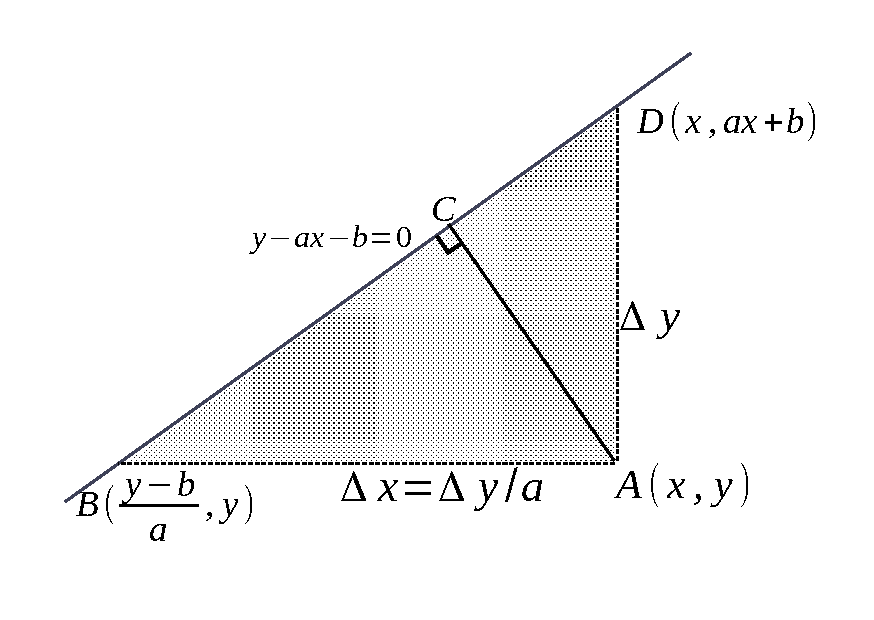
\includegraphics[width=8cm]{./image/16_/RegressionModel.pdf}
  \caption{点$A$と直線$Y=aX+b$の関係}
  \label{fig:RegressionModel}
 \end{center}
\end{figure}

以上から点と直線の距離について4つの方法で定義ができることがわかる。
また、各点についてそれぞれの式を和にすると、以下の通りである。
\begin{enumerate}
 \item 点と直線の最短距離$AC$:$E_3 = \sum (\frac{\Delta y_i}{\sqrt{1+a^2}})^2$
 \item $y$軸に関する距離$AD$:$E_1=\sum \Delta y_i^2$
 \item $x$軸に関する距離$AB$:$E_2=\sum  (\frac{\Delta y_i}{a})^2=\sum (\Delta x)^2$
 \item 面積を元にした距離$AB\times AD$:$2\times E_4 = \sum (\frac{\Delta y_i}{\sqrt{a}})^2$
\end{enumerate}

ある点と直線への距離が離れていれば、その点への予測ができていないことを示し、近ければ、それなりによい予測をしているだろう。
このことから、$E_j$が小ければ、それぞれの距離の意味で、各々の点と直線が近いはずである。
そこで、まず$E_j$が最も小さくなるように直線のパラメータ$(a_j,b_j)(j=1,2,3,4)$を定める。
さらに、それぞれの直線の性質についてしらべる。


\paragraph{点と直線の最短距離}
点と直線の距離について証明を行う。大抵の高校数学の教科書には記述されているはずである。
点$A(x,y)$から直線$Y-aX-b=0$への直線距離$d$の関係を求める。
点$B$は、点$A$を$x$方向に移動させたとき、直線と交わる点である。つまり点$B$は、$(\frac{y-b}{a},y)$である。
また点$D$は、点$A$を$y$方向に移動させたとき、直線と交わる点である。つまり点$D$は、$(x,ax+b)$である。
点$C$は、点$A$を直線$Y-aX-b=0$へ垂直に下ろした点である。この$AC$間の距離を$d$とする。
直線$DA$と直線$AC$のなす角度を$\theta$とする。
このとき、次の関係が求められる。
\begin{eqnarray*}
 \sin \theta &=& \frac{AC}{BA}\\
 &=& \frac{d}{x-\frac{y-b}{a}}\\
\cos\theta &=& \frac{AC}{DA}\\
&=& \frac{d}{ax+b-y}
\end{eqnarray*}
また、$\cos^2\theta+\sin^2\theta$を計算する。
\begin{eqnarray*}
 \cos^2\theta+\sin^2\theta &=& \frac{d^2}{(y - \frac{y-b}{a})^2}+\frac{d^2}{(ax+b-y)^2}\\
 &=& \frac{d^2(a^2+1)}{(ax+b-y)^2} \\
 &=& 1
\end{eqnarray*}
この式を$d$について解く。
\begin{equation*}
 d^2 = \frac{(y-ax-b)^2}{a^2+1}
\end{equation*}


\begin{figure}
 \begin{center}
  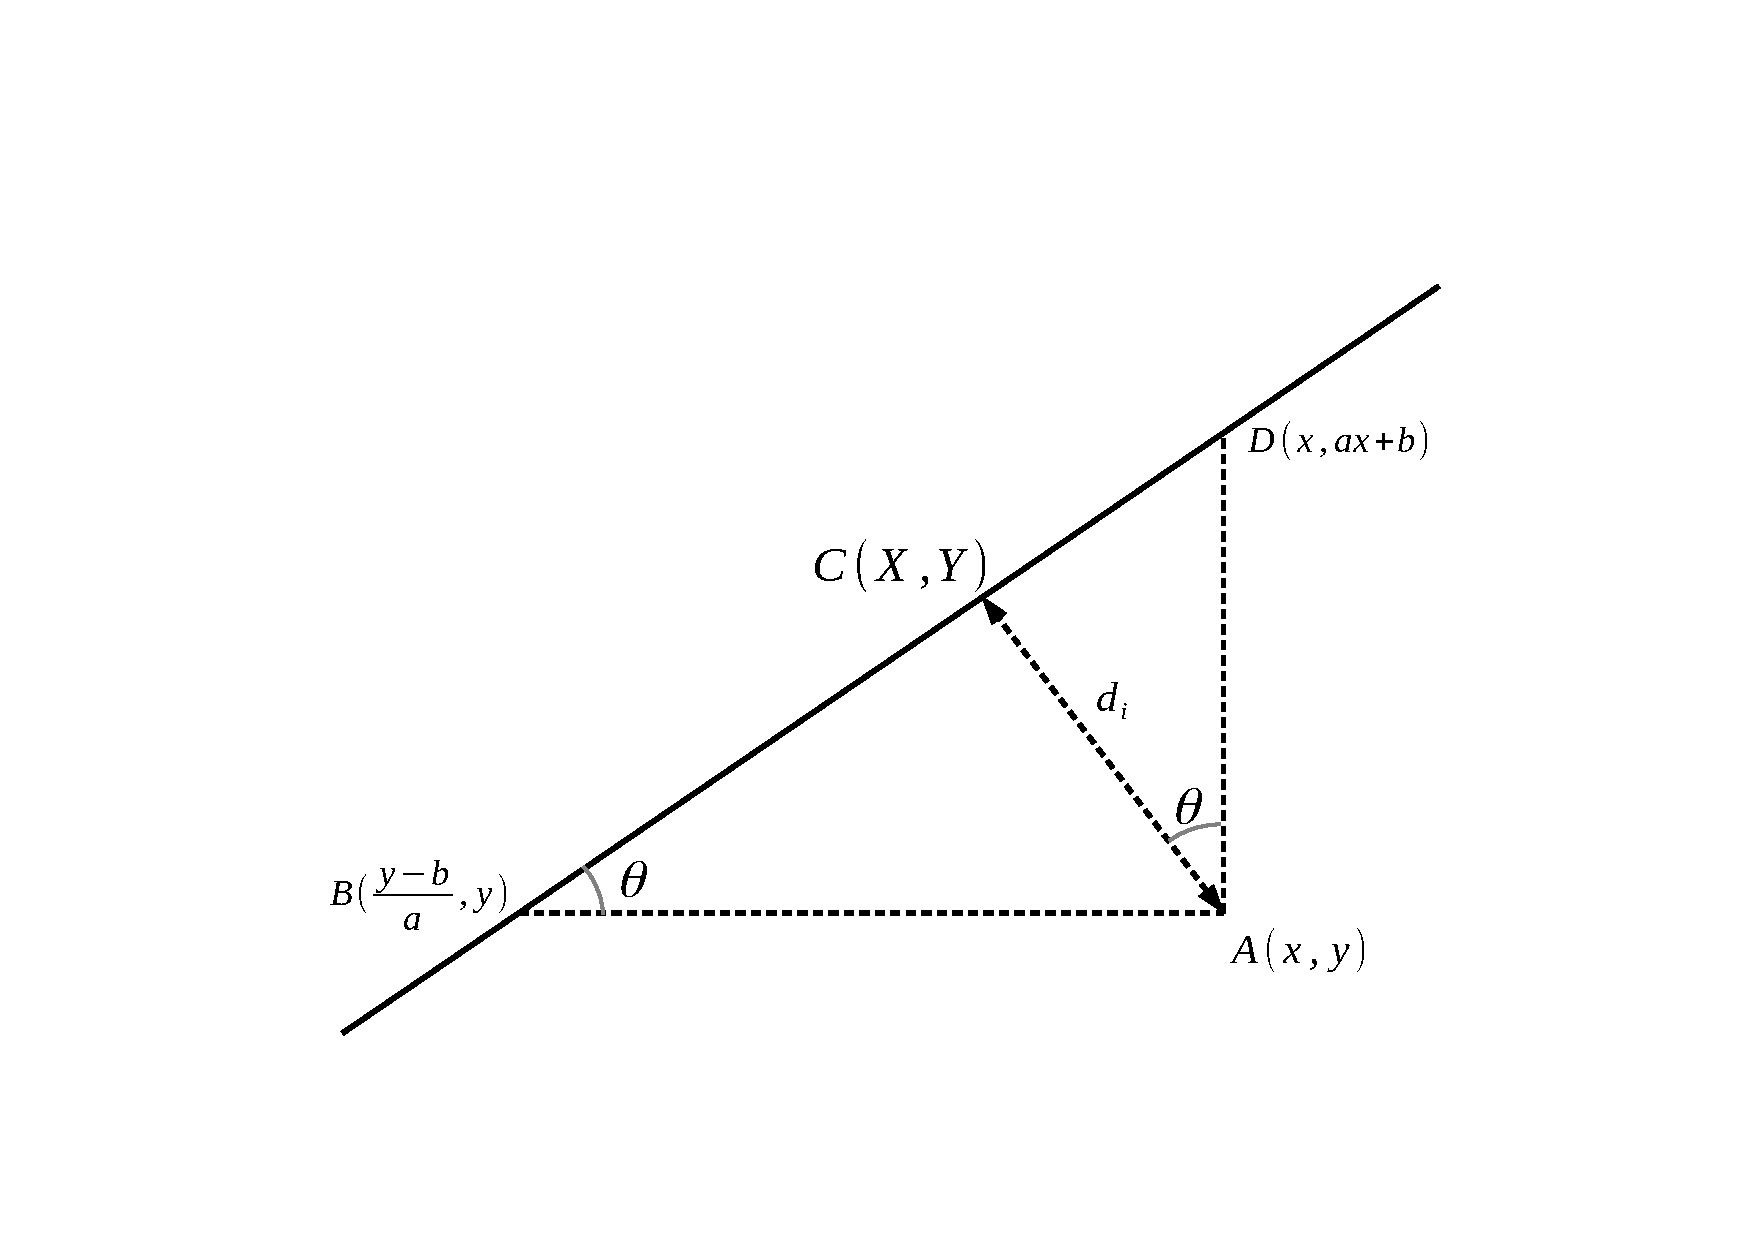
\includegraphics[width=8cm]{./image/16_/point_line_distance.pdf}
  \caption{点$A$から直線$Y=aX+b$への直線距離$d$の関係}
  \label{fig:point_line_distance}
 \end{center}
\end{figure}

\paragraph{$\sum \Delta y_i^2$に関する計算}
\begin{equation}\label{sum_square_error}
 E_1 = \sum_{i=1}^n u_i^2 = \sum_{i=1}^n (y_i-a x_i-b)^2
\end{equation}
式\ref{sum_square_error}にいくらか式変形を行う。
\begin{eqnarray*}
 \sum_{i=1}^n (y_i-a x_i-b)^2 &=& \sum_{i=1}^n \{(y_i-\bar{y}) - a(x_i-\bar{x}) +(\bar{y}-b-a\bar{x})  \}^2\\
 & =& \sum_{i=1}^n \{ (y_i-\bar{y})-a(x_i-\bar{x})  \}^2+n(\bar{y}-b-a\bar{x})^2 \\
 &=& Q^2_{xx}a^2-2Q_{xy}a+Q^2_{yy}+n(\bar{y}-b-a\bar{x})^2
\end{eqnarray*}
ここで、以下の式を定義しておく。
\begin{eqnarray*}
 \bar{x} &=& \frac{1}{n}\sum_{i=1}^n x_i \\
 \bar{y}&=& \frac{1}{n}\sum_{i=1}^n y_i \\
 Q^2_{xx} &=& \sum_{i=1}^n (x_i-\bar{x})^2 \\
 Q^2_{yy} &=& \sum_{i=1}^n (y_i-\bar{y})^2 \\
 Q_{xy} &=& \sum_{i=1}^n (x_i-\bar{x})(y_i-\bar{y}) \\
\end{eqnarray*}

\paragraph{$E_1$}
まず、式\ref{sum_square_error}を、$b$について偏微分を行う。
\begin{equation*}
 \frac{\partial E_1}{\partial b} = -2(\bar{y}-b-a\bar{x})
\end{equation*}
この式が$0$となる$b$について解くと、次が求まる。
\begin{equation*}
 \hat{b} = \bar{y}-\hat{a}\bar{x}
\end{equation*}

また、$E_1$を$a$について偏微分を行う。
\begin{eqnarray*}
 \frac{\partial E_1}{\partial a} = 2aQ^2_{xx}-2Q_{xy}
\end{eqnarray*}
以上から、$a$が求められる。
\begin{equation*}
 \hat{a} = \frac{Q_{xy}}{Q^2_{xx}}
\end{equation*}


\paragraph{$E_2$}
$a,b$に関係する部分は、以下の式である。
\begin{equation*}
 E_2 = \frac{1}{a^2}(Q^2_{xx}a^2-2Q_{xy}a+Q^2_{yy}+n(\bar{y}-b-a\bar{x})^2)
\end{equation*}
$E_2$の$b$に関する偏微分が$0$になる点は、以下の式である。
\begin{equation*}
 \hat{b} = \bar{y}-\hat{a}\bar{x}
\end{equation*}
また、$E_2$の$a$に関する偏微分を計算する。
\begin{eqnarray*}
 \frac{\partial E_2}{\partial a} &=& -\frac{2}{a^3}(a^2Q^2_{xx}-2Q_{xy}a+Q^2_{yy}) \\
& & +\frac{1}{a^2}(2aQ^2_{xx}-2Q_{xy})
\end{eqnarray*}
この式を$a$についてとくと、最尤推定量がもとめられる。
\begin{equation*}
 \hat{a}= \frac{Q^2_{yy}}{Q_{xy}}
\end{equation*}

\paragraph{$E_3$}

変数$a,b$に関連のある項を計算する。
\begin{eqnarray*}
 h(a,b) = \sum_{i=1}^n (x_i-u_i)^2+(y_i-v_i)^2
\end{eqnarray*}
対数尤度を最大化するかつ$v_i -a u_i -b = 0$を満すものを求める。

これは難しいので、幾何学的な考察を行う。
$h(a,b)$は、$(x_i,y_i)$から$(u_i,v_i)$上への距離の和を示している。これを最小化するのは、$(x_i,y_i)$から直線$v_i-a u_i-b=0$への直線距離を最小化しているのに等しい。
このことから、直線から点への距離の公式から、その和は、次の式で表すことができる。
\begin{equation*}
 E_3 = \sum_{i=1}^n \frac{ (y_i-b-ax_i)^2}{1+a^2}
\end{equation*}
$E_1$との違いは、分母に$(1+a^2)$の項が加わったことである。これが、推定量に違いを生じさせる。
式$E_3$を展開していく。
\begin{comment}
\begin{eqnarray*}
 (1+a^2)E_3 &=& \sum_{i=1}^n \{ (y_i-\bar{y})-a(x_i-\bar{x})+(\bar{y}-a\bar{x}-b) \}^2 \\
 &=& \sum_{i=1}^n \{  (y_i-\bar{y})-a(x_i-\bar{x}) \}^2+n(\bar{y}-a\bar{x}-b)^2 \\
 &=& Q^2_{yy}+a^2 Q^2_{xx}-2aQ_{xy}+n(\bar{y}-a\bar{x}-b)^2 \\
\end{eqnarray*} 
\end{comment}


\begin{equation*}
 (1+a^2)E_3 = Q^2_{yy}+a^2 Q^2_{xx}-2aQ_{xy}+n(\bar{y}-a\bar{x}-b)^2 \\
\end{equation*}
この式を最小化する。まず$b$により偏微分を行う。
\begin{eqnarray*}
 \frac{\partial E_3}{\partial b} = -2n(\bar{y}-a\bar{x}-b)
\end{eqnarray*}
これが$0$になるので、最尤推定した$\hat{b}$は次の式となる。
\begin{equation*}
 \hat{b} = \bar{y}-\hat{a}\bar{x}
\end{equation*}
次に、$a$について偏微分をおこなう\footnote{ $(f/g)'= \frac{f'g-fg'}{g^2}$ }。
\begin{eqnarray*}
\frac{\partial E_3}{\partial a} = \frac{(2aQ^2_{xx}-2Q_{xy})(1+a^2)-2a(Q^2_{yy}+a^2Q^2_{xx}-2aQ_{xy})}{(1+a^2)^2}
\end{eqnarray*}
分子を整理すると、次の式となる。
\begin{equation*}
 Q_{xy}a^2-a(Q^2_{yy}-Q^2_{xx})-Q_{xy}
\end{equation*}
$\frac{\partial E_3}{\partial a} =0$より、$a$について解く。
上式は、$a$に関する二次方程式なので、$a$を解く。
\begin{equation*}
 \hat{a} = \frac{Q^2_{yy}-Q^2_{xx}+\sqrt{(Q^2_{yy}-Q^2_{xx})^2+4Q_{xy}}}{2Q_{xy}}
\end{equation*}




\paragraph{$E_4$}
\begin{eqnarray*}
 E_4=\sum_{i=1}^n u_i^2 &=& \sum_{i=1}^n \frac{1}{a}(y_i-a x_i-b)^2 \\
 &=& \frac{1}{a}(Q^2_{xx}a^2-2Q_{xy}a+Q^2_{yy}+n(\bar{y}-b-a\bar{x})^2)
\end{eqnarray*}
ここで、$E_4$の$b$に関する偏微分が$0$となる$b$を求める。
\begin{equation*}
 \hat{b} = \bar{y}-\hat{a}\bar{x}
\end{equation*}
同様に、$E_4$の$a$に関する偏微分が$0$となる$a$を求める。
\begin{eqnarray*}
 \frac{\partial E_4}{\partial b} &=& \frac{1}{a}(2aQ^2_{xx}-2Q_{xy})\\
&& -\frac{1}{a^2}(Q^2_{xx}a^2-2Q_{xy}a+Q^2_{yy}) = 0 \\
\rightarrow && a^2 Q^2_{xx}-Q^2_{yy} = 0
\end{eqnarray*}
以上から、最尤推定量が求められる。
\begin{equation*}
 \hat{a}= \sqrt{\frac{Q^2_{yy}}{Q^2_{xx}}}
\end{equation*}
この式は、$\frac{Q_{xy}}{Q^2_{xx}}$と$\frac{Q^2_{yy}}{Q_{xy}}$の幾何平均と一致する。
ここで、幾何平均は、$0$より大きな数$a_1,a_2,\cdots,a_n$について、次の量のことである。
\begin{equation*}
 (a_1a_2\cdots a_n)^{\frac{1}{n}}
\end{equation*}

\subsection{傾きの大小関係}
実際のところ、$E_1$の中にも$a$に係る項が入っているので、$a$がどのような値になるかは推測しにくい。気持ちとして以下のようになることが考えられる。
$E_2,E_3$は、分母に傾き$a$が入っている。この項が$1$より大きければ、$E_2,E_3$を小くし、$1$より小ければ、$E_2,E_3$は大きくなる。
このことから、$E_2,E_4$において$a$は$1$よりも大きくなりがちであることが予想される。
$E_3$については、分母に$1+a^2$の項があるため、任意の$a$において、$E_3$を小くしてくれそうである。

\paragraph{$a_1$と$a_2$の大小関係}
\begin{eqnarray*}
 \frac{1}{a_2}a_1 &=& \frac{Q_{xy}}{Q^2_{yy}}\frac{Q_{xy}}{Q^2_{xx}} \\
 &=& \frac{Q_{xy}}{Q^2_{xx}Q^2_{yy}}
\end{eqnarray*}
ここで、$r^2$を以下のように定める。
\begin{equation*}
 r^2 = \frac{Q_{xy}}{Q^2_{xx}Q^2_{yy}}
\end{equation*}
この$r^2$は$1$以下であることから、
\begin{equation*}
 a_1 \leq a_2
\end{equation*}
であることがわかる。
これは、$E_2$の直線の傾きは$E_1$の直線の傾きよりも急であることを示唆している。

\paragraph{$a_1,a_2,a_4$の関係}
相加相乗平均とは次のことである。
実数$a,b>0$について、次が成り立つ。
\begin{equation*}
 \frac{a+b}{2} \geq \sqrt{ab}
\end{equation*}

ここで、$a=a_1,b=a_2$とおくと次がわかる。
\begin{equation*}
 \frac{a_1+a_2}{2}  \geq  \sqrt{a_1 a_2} = a_4
\end{equation*}
このことから、$a_4$は$a_1,a_2$の平均値よりも小さい。



\begin{table}[http]
 \centering
 \begin{tabular}{lcc}
  & a & b\\
  \hline 
  $E_1$ & $\frac{Q_{xy}}{Q^2_{xx}}$  &$\bar{y}-\hat{a}\bar{x}$ \\
  $E_2=\frac{1}{a^2}E_1$ & $\frac{Q^2_{yy}}{Q_{xy}}$ & $\bar{y}-\hat{a}\bar{x}$ \\
$E_3=\frac{1}{1+a^2}E_1$ & $\frac{Q^2_{yy}-Q^2_{xx}+\sqrt{(Q^2_{yy}-Q^2_{xx})^2+4Q_{xy}^2}}{2Q_{xy}}$ & $\bar{y}-\hat{a}\bar{x}$ \\
  $E_4=\frac{1}{a}E_1$ & $\sqrt{\frac{Q^2_{yy}}{Q^2_{xx}}}$ & $\bar{y}-\hat{a}\bar{x}$
 \end{tabular}
\end{table}

\if 0 
https://cdnsciencepub.com/doi/full/10.1139/Z10-050
https://davegiles.blogspot.com/2014/11/orthogonal-regression-first-steps.html
https://www2.clarku.edu/faculty/pbergmann/biostats/McArdle%201988.pdf
https://qiita.com/HiroyukiTachikawa/items/cc2f48161e4da8da69f1
https://pdodds.w3.uvm.edu/files/papers/others/2006/warton2006a.pdf
https://research.usq.edu.au/download/3fd0a55ab4c8c0e70af81c9b4ba9b015175b8908c54d0891c48bbe1946e9f7c0/1087797/Saqr_Khan_ICCS2012_PV.pdf
https://www.jstage.jst.go.jp/article/jscc1971b/27/1/27_21/_pdf
https://twitter.com/fronori/status/939418738406727680
https://www.jstage.jst.go.jp/article/jjshwr/16/3/16_3_284/_pdf
https://biolab.sakura.ne.jp/sma-regression.html
https://biolab.sakura.ne.jp/regression-correlation.html
https://home.iitk.ac.in/~shalab/econometrics/Chapter2-Econometrics-SimpleLinearRegressionAnalysis.pdf
https://home.iitk.ac.in/~shalab/course3.htm



https://twitter.com/uncorrelated/status/1728243372002058681

PyMC
https://zenn.dev/yoshida0312/articles/f5579f88e22b22#%E3%83%87%E3%83%BC%E3%82%BF%E3%81%AE%E6%BA%96%E5%82%99-1
https://www.pymc.io/projects/docs/en/v3.11.4/pymc-examples/examples/generalized_linear_models/GLM-robust-with-outlier-detection.html
https://qiita.com/TomokIshii/items/a62a03a6a0456a813fa7
https://zenn.dev/yoshida0312/articles/8f10d1380b4d98
https://discourse.pymc.io/t/errors-in-variables-model-in-pymc3/3519
https://github.com/pymc-devs/pymc/issues/2226
https://learning-with-machine.hatenablog.com/entry/2020/10/01/193000
https://twitter.com/hankagosa/status/1727264718451261868
https://stats.stackexchange.com/questions/431359/how-to-find-the-best-fit-line-in-this-case

https://work-in-progress.hatenablog.com/entry/2018/11/17/074452

\fi



\chapter{親子の身長の関係/予測}
\section{Galtonによる親子の身長の研究}
Galtonは両親と子供の身長について計測をおこない、これを解析した。
オリジナルのデータが残っており、2004年にノートから数値データが得られている\footnote{\url{https://vincentarelbundock.github.io/Rdatasets/doc/HistData/GaltonFamilies.html}}。
各家庭の子供の個体数は$1-15$人であり、その分布は図\ref{fig:Galton_child_parent_num}に示した通りである。
205家庭から、963人の子供の身長を計測した。男女の内分けは、486人が息子、476人が娘である。
934人については、身長が数値で記録されており、残りの29人については言葉で、tallish,middle,deformed,idioticなどと記載されている。
Galtonの論文から得られたデータは\footnote{\url{https://vincentarelbundock.github.io/Rdatasets/doc/HistData/Galton.html}}、親と子のペアは$928$点となっており、オリジナルデータからいくつかが抜かれている。Galtonがどのデータを省いたのかを特定するのは難しい。
今回は、ノート記載されている934人の子供の身長を解析する。身長の単位はインチで記録されているので、$2.54$倍しセンチメートルに書き換えた。

\begin{figure}
 \begin{center}
  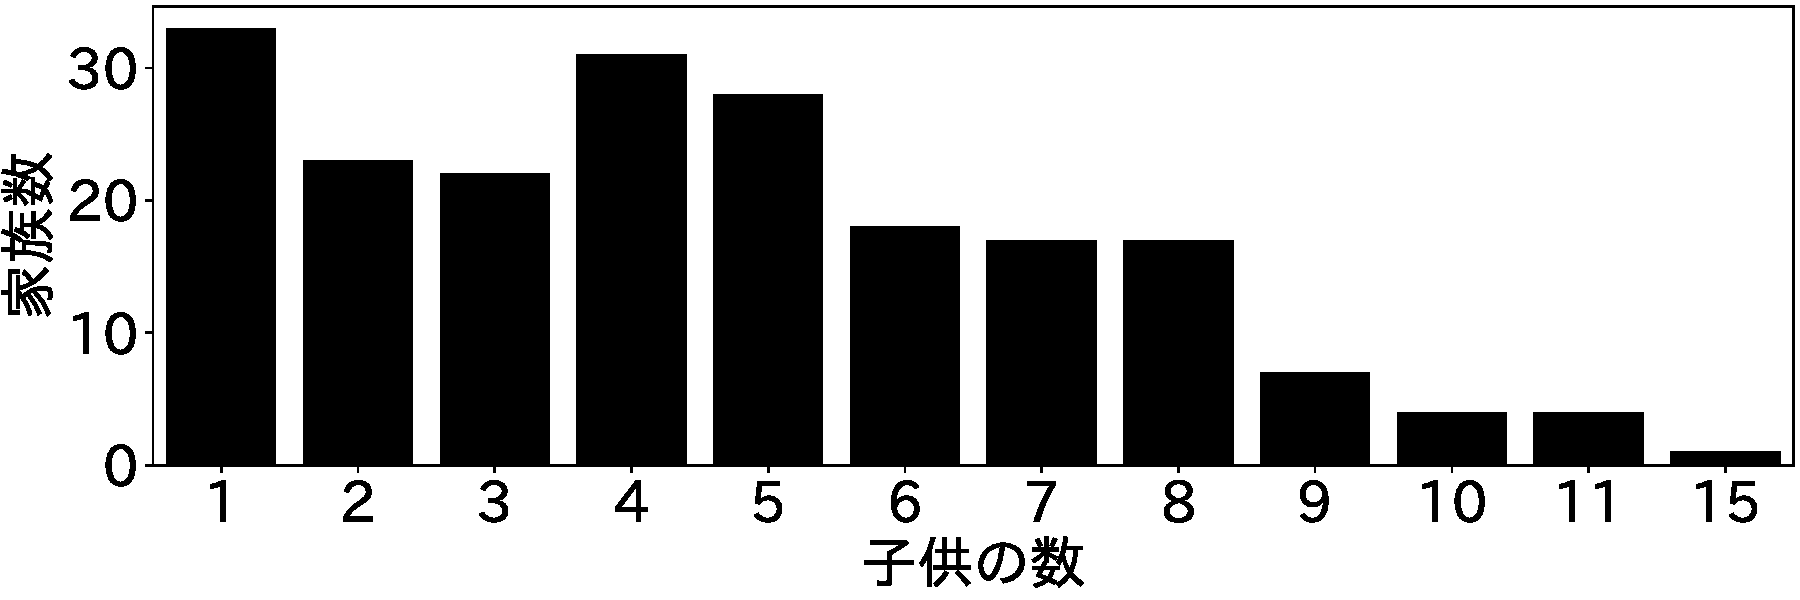
\includegraphics[width=10cm]{./image/16_/Galton/Galton_data_num_child.pdf}
  \label{fig:Galton_child_parent_num}
  \caption{子供の数と家族の数に関する分布}
 \end{center}
\end{figure}


\begin{table}[http]
 \centering \caption{}
\begin{tabular}{lrrrrrrr}
 & 息子 & 娘 & 補正娘 & 補正子供 & 中間親 & 父親 & 母親 \\
該当個数 & 481 & 453 & 453 & 934 & 205 & 205 & 205 \\
平均 & 175.85 & 162.82 & 175.85 & 175.85 & 175.82 & 176.06 & 162.56 \\
標準偏差 & 6.66 & 5.98 & 6.46 & 6.56 & 4.86 & 6.72 & 5.93 \\
最小値 & 152.40 & 142.24 & 153.62 & 152.40 & 163.58 & 157.48 & 147.32 \\
$25\%$ & 171.45 & 158.75 & 171.45 & 171.45 & 172.77 & 172.72 & 160.02 \\
$50\%$ & 175.77 & 162.56 & 175.56 & 175.56 & 175.72 & 176.53 & 162.56 \\
$75\%$ & 180.34 & 166.37 & 179.68 & 180.34 & 178.79 & 180.34 & 166.37 \\
最大値 & 200.66 & 179.07 & 193.40 & 200.66 & 191.59 & 199.39 & 179.07 \\
\end{tabular}
\end{table}

\subsection{データのモデルへの適合具合}

図\ref{fig:Galton_midparent_cumhist},\ref{fig:Galton_male_female_cumhist}には、中間親の身長、子供の身長の経験累積分布を示した。
それぞれの変量はそれなりに正規分布にしたがっていることがわかる。

最尤推定モデルの中心と身長ペアの間のマハラノビス距離を計算し、その経験累積分布を図\ref{fig:Galton_Mahalanobis_distance_distribution}に示した。
マハラノビス距離は理論通りであれば$t^2$分布にしたがい、経験分布をみるとそれなりに$t^2$分布にしたがっている。
身長のペアが2変量モデルに適合的であることがわかる。


\begin{figure}
 \begin{center}
  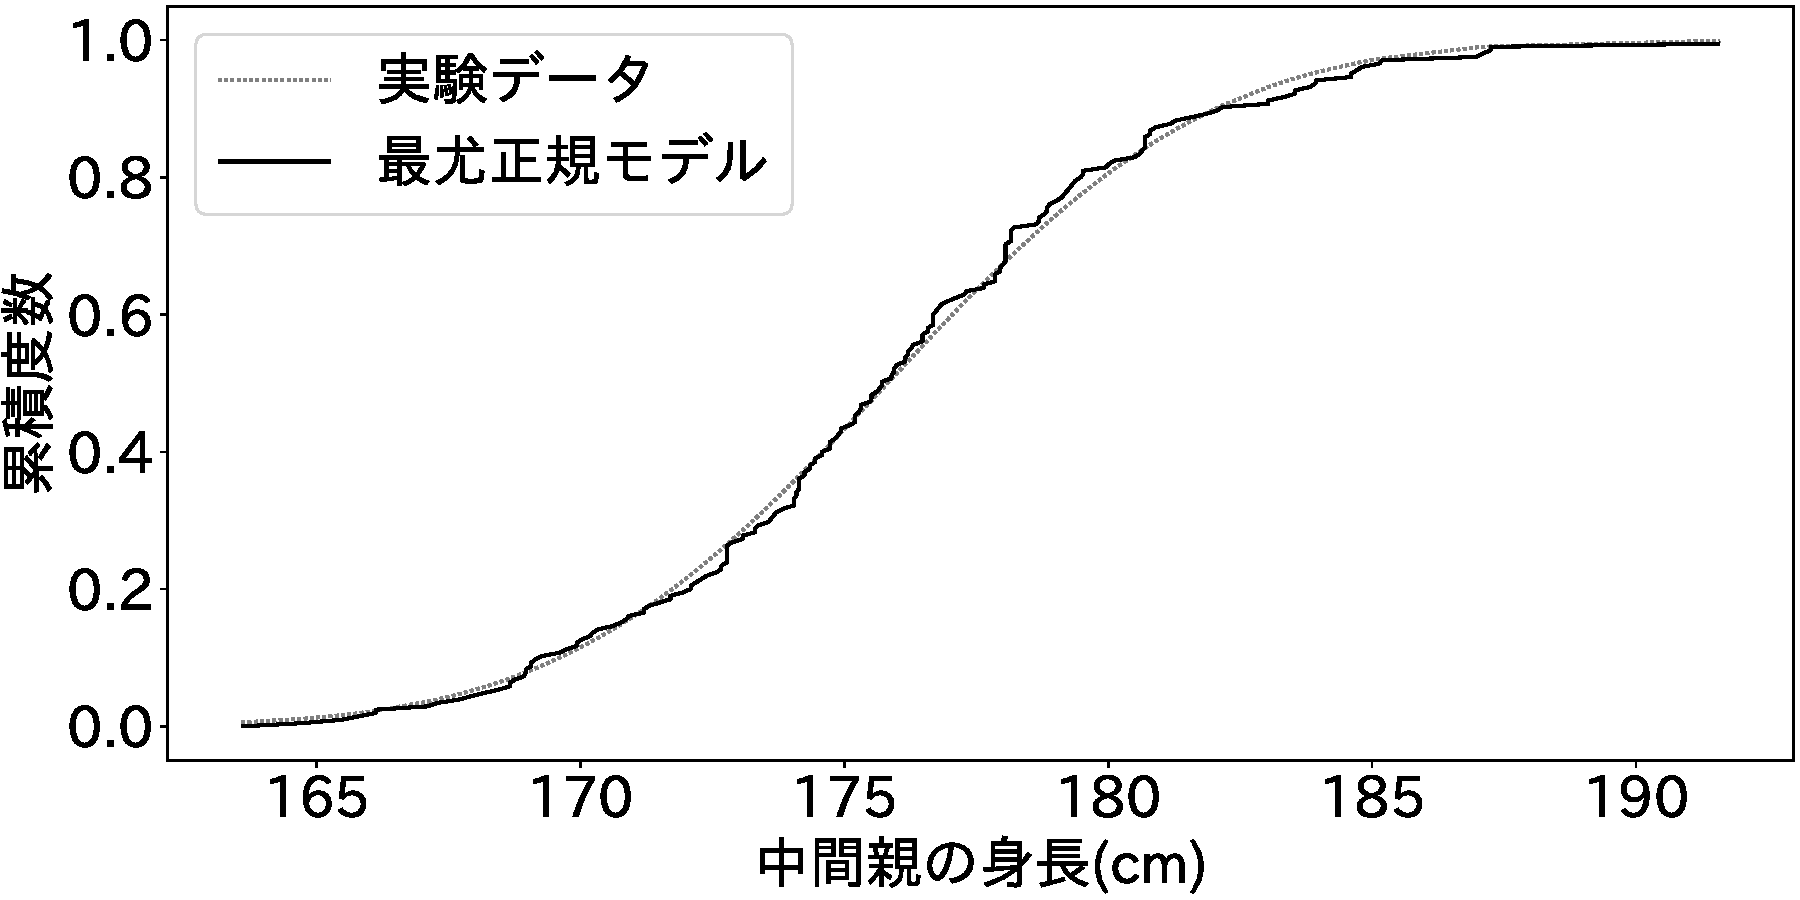
\includegraphics[width=10cm]{./image/16_/Galton/midparent_cumhist.pdf}
  \label{fig:Galton_midparent_cumhist}
  \caption{中間親の身長の累積度数分布}
 \end{center}
\end{figure}

\begin{figure}
 \begin{center}
  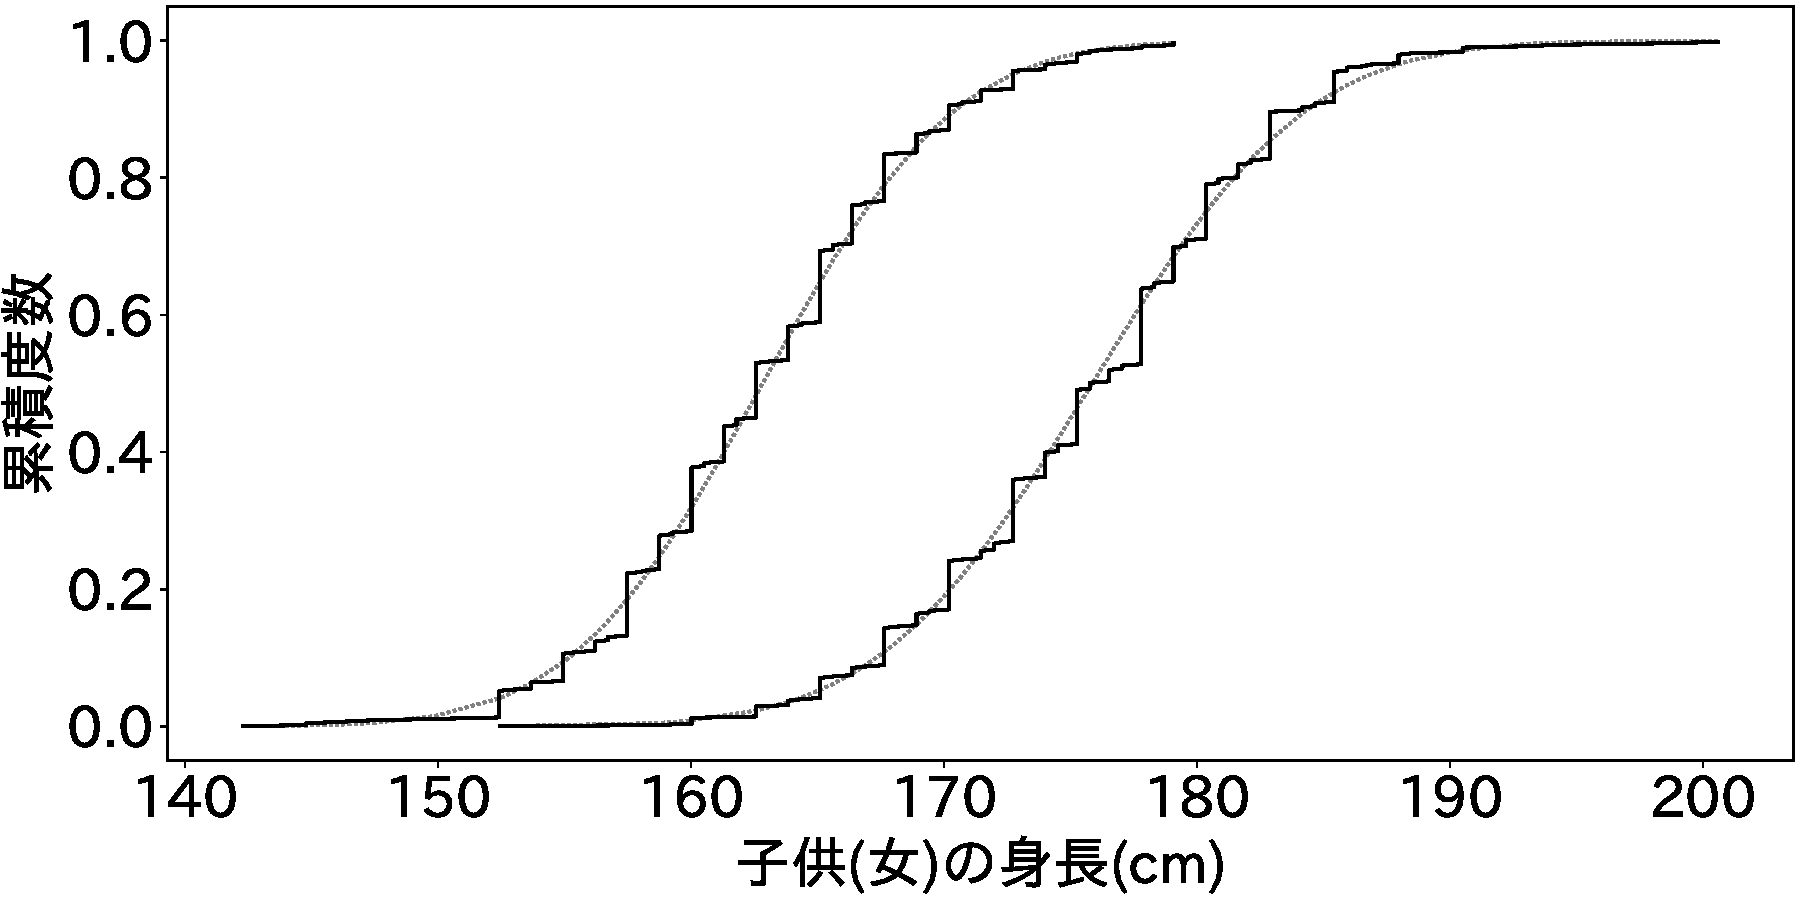
\includegraphics[width=10cm]{./image/16_/Galton/male_female_cumhist.pdf}
  \label{fig:Galton_male_female_cumhist}
  \caption{男と女の身長の累積度数分布}
 \end{center}
\end{figure}


\begin{figure}
 \begin{center}
  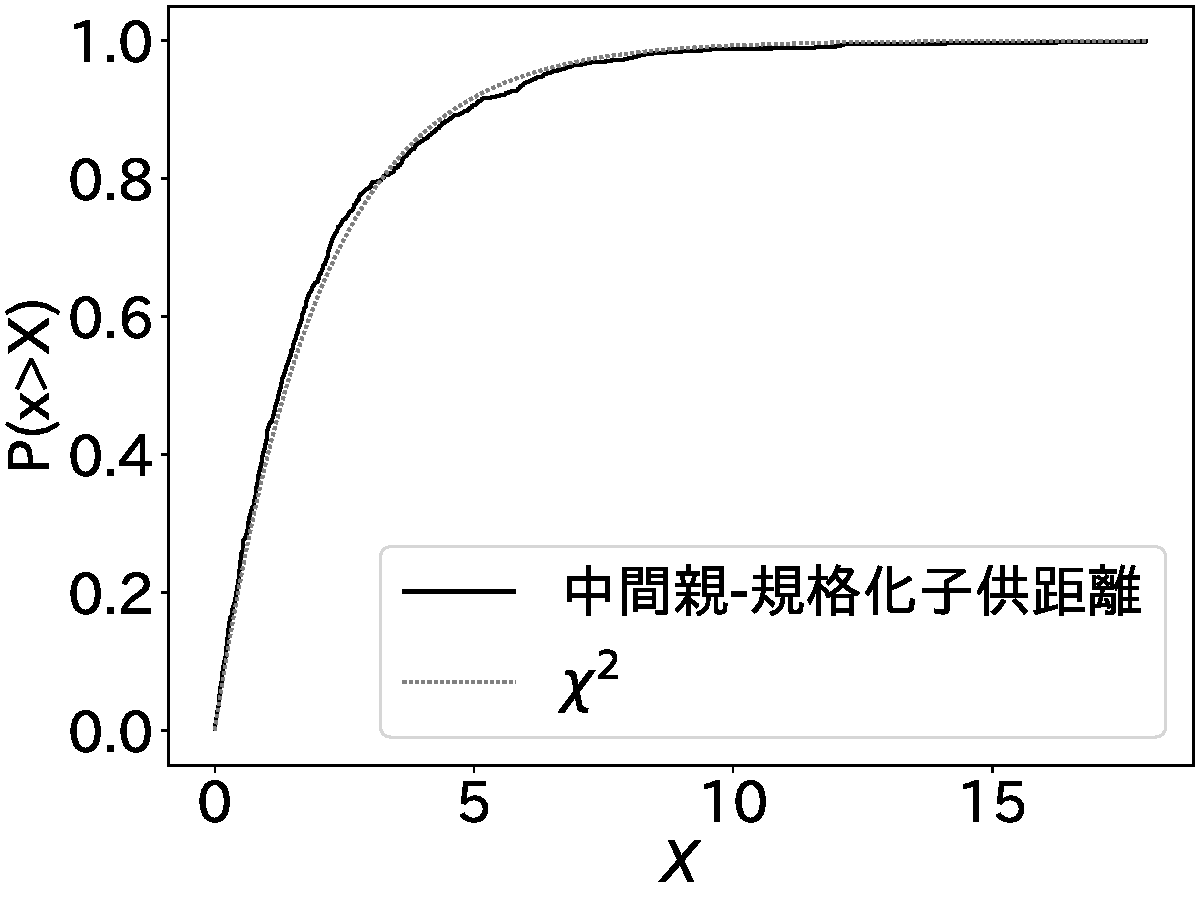
\includegraphics[width=10cm]{./image/16_/Galton/Galton_Mahalanobis_distance_distribution.pdf}
  \label{fig:Galton_Mahalanobis_distance_distribution} \caption{中間親と規格化子供の間のマハラノビス距離}
 \end{center}
\end{figure}

\subsection{回帰/主軸}


\begin{figure}
 \begin{center}
  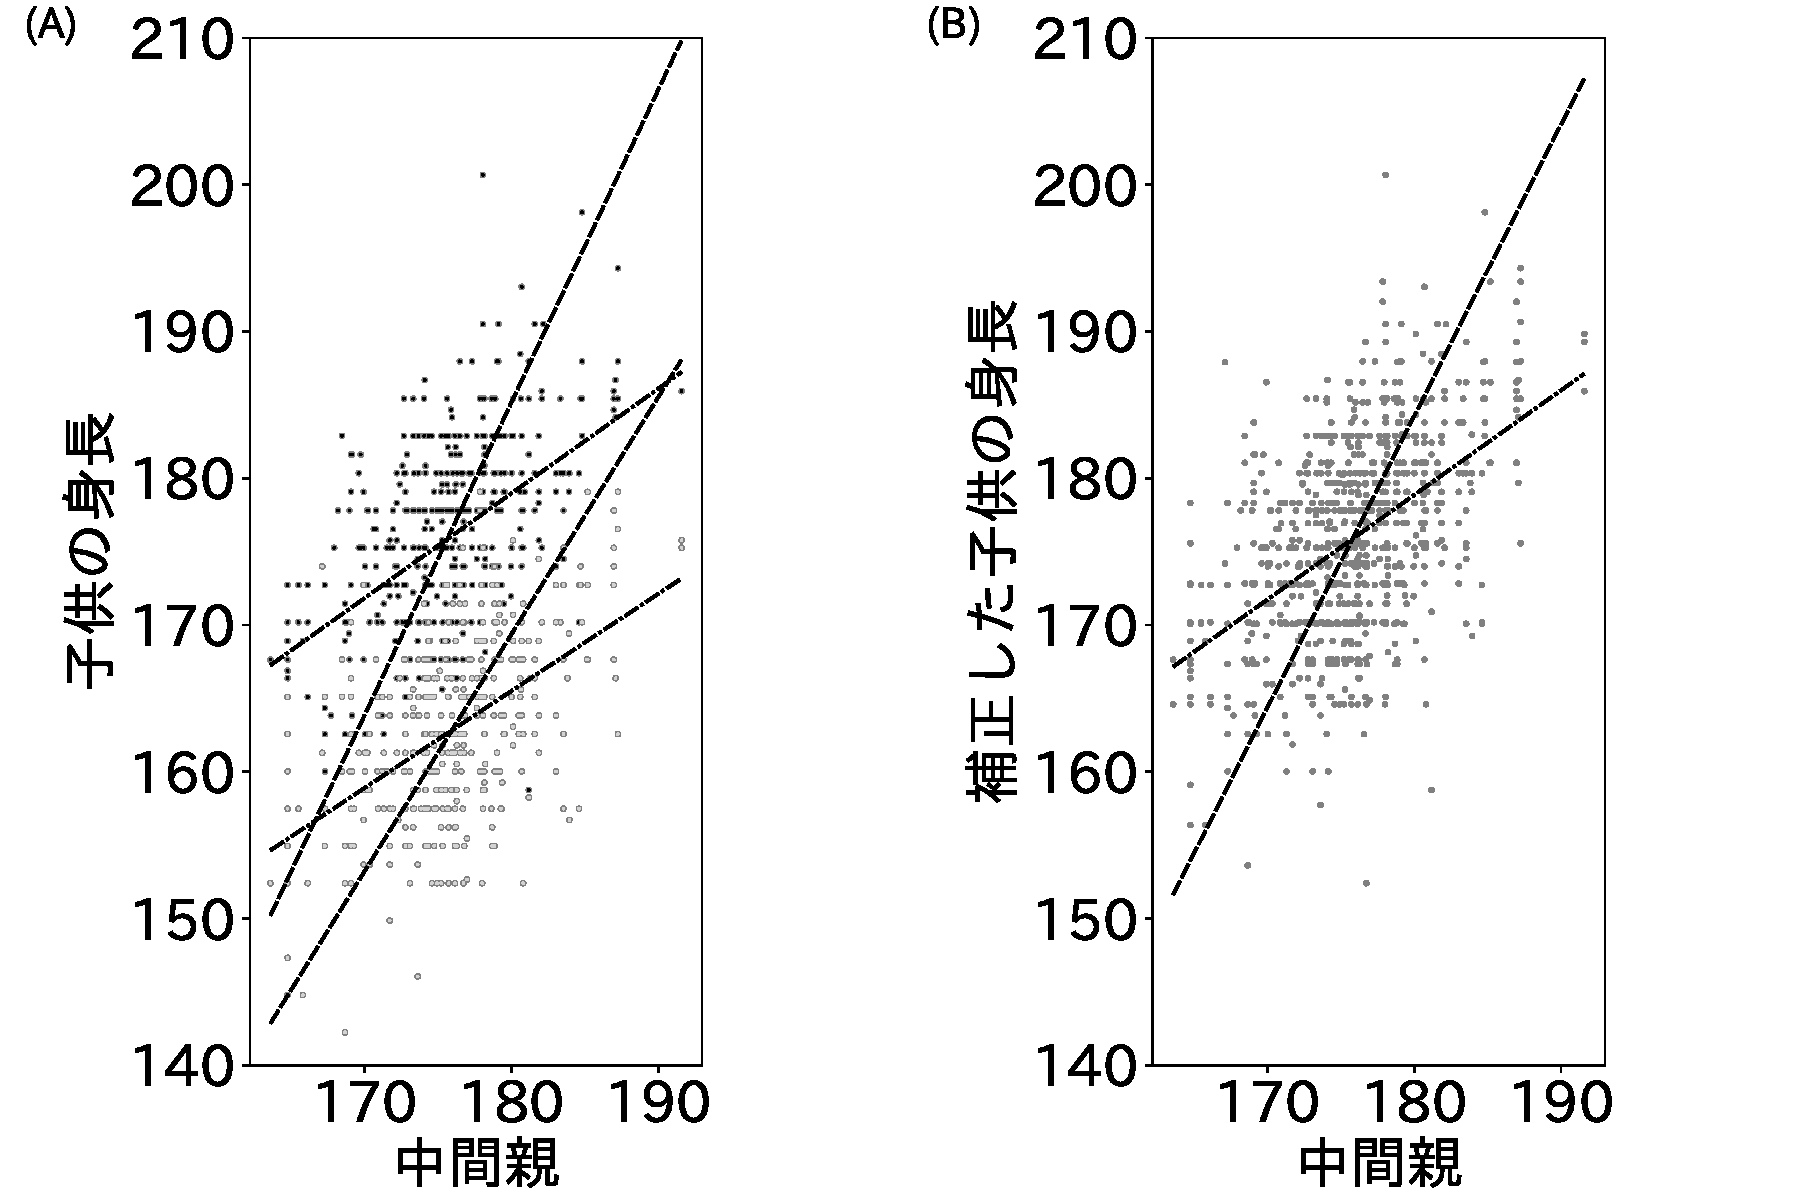
\includegraphics[width=10cm]{./image/16_/Galton/male_female_scatter.pdf}
  \label{fig:Galton_male_female_scatter} \caption{男と女の身長の散布図。(A)息子(黒色の点)または娘(灰色の点)と中間親との散布図。(B)娘に1.08倍の補正をした身長と中間親の身長の散布図。一点鎖線が回帰直線、破線がPCAの直線。}
 \end{center}
\end{figure}

\begin{table}[http]
 \centering \caption{中間親と子供との相関係数($\rho$)、決定係数($R^2$)、誤差($RMSE$)、傾き($a_1,a_3$)}
\begin{tabular}{lccccc}
 & $\rho$ & $R^2(=\rho^2)$ & RMSE & $a_1$ &$a_3$ \\
子供の男女区別無し & 0.32 & 0.10 & 8.61 & 0.64 & 4.83 \\
子供の男女区別無し(娘の身長$\times 1.08$) & 0.50 & 0.25 & 5.69 & 0.71& 1.98 \\
娘 & 0.51 & 0.26 & 5.13 & 0.66 & 1.61 \\
息子 & 0.48 & 0.23 & 5.83 & 0.71 & 2.13 \\
\end{tabular}
\end{table}




\if 0
\section{PearsonとLee}
PearsonとLeeらによる親と子供の身長に関するデータを利用した\footnote{\url{https://vincentarelbundock.github.io/Rdatasets/datasets.html}}。
\begin{table}[http]
 \centering
 %父と息子の統計量を要約したもの
 \begin{tabular}{lrr}
  {} &  子供 &  親 \\
  個数 & 179 &  179 \\
  平均  &  68.33 &   67.08 \\
  標準偏差   &   4.53 &    4.03 \\
  最小値   &  59.50 &   58.50 \\
  25\%   &  64.50 &   64.00 \\
  50\%   &  68.50 &   67.50 \\
  75\%   &  71.50 &   70.50 \\
  最大値   &  78.50 &   74.50 \\
 \end{tabular}
\end{table}


\begin{table}[http]
 \centering
\begin{tabular}{lrr}
{} &    $\hat{a}$ &      $\hat{b}$ \\
$E_1$ & 0.59 &  29.02 \\
 $E_2$ & 2.16 & -76.69 \\
$E_3$ & 1.25 & -15.76 \\
$E_4$ & 1.13 &  -7.18 \\
\end{tabular}
\end{table}
\fi


\chapter{回帰モデル}


\section{誤差モデルI}
ここで、誤差項が確率変数であることを仮定してモデルModel Iを構築する。
\begin{enumerate}
 \item $x_i$は、与えられた定数
 \item $a,b$を実数の定数
 \item $u_i = y_i-a x_i -b$
 \item $u_i \sim N(0,\sigma^2)$
 %\item $E[u_i]=0$。平均は$0$。
 %\item $E[u_j u_i]=0$。無相関。
 %\item $Var[u_i]=0$。分散が均一。
\end{enumerate}
この仮定により構築されるモデルを$M_{I}(a,b; x)$または$M_I(a,b)$と表記する\footnote{正規性の仮定の代わりに、無相関、等しい分散、平均が$0$の仮定を与えるのが簡単な定義である。ここでは、正規性を仮定しておいた}。
また、最尤推定量を挿入した最尤モデルを$M_I(\hat{a},\hat{b})$と表記する。
この最尤推定量は次の通りである。
\begin{eqnarray*}
 \hat{a} &=& \frac{Q_{xy}}{Q^2_{xx}}\\
 \hat{b} &=& \bar{y}-\hat{a}\bar{x}
\end{eqnarray*}
予測値と観測値の差分を残差$e_i$、またその二乗和を残差平方和とよぶ。それぞれ、以下の通り。
\begin{eqnarray*}
 e_i &=& y_i - (ax_i+b)\ \ (i=1,2,\cdots,n)\\
 RSS &=& \sum_{i=1}^n e_i^2 \\
\end{eqnarray*}
そして分散の推定値を以下のように定義する。
\begin{eqnarray*}
 \hat{\sigma}^2 = \frac{RSS}{n-2}
\end{eqnarray*}
モデル$M_I(a,b)$において、次のことも解っている。
\begin{equation*}
 \frac{(\hat{a}-a)}{ \left( \frac{\hat{\sigma}^2}{Q^2_{xx}} \right)^\frac{1}{2}} \sim t_{n-2}
\end{equation*}
また、このことから、$a$の信頼区間は、次の通り。
\begin{equation*}
 |a| \leq \hat{a}\pm(\hat{\sigma}^2/Q^2_{xx})^{1/2}t_{n-2,\frac{\alpha}{2}}
\end{equation*}
$y$の予測区間は、以下の通りである。
\begin{equation*}
 y_0\pm\left[\hat{\sigma}^2\left( 1+\frac{1}{n} +\frac{(x_0-\bar{x})^2}{Q^2_{xx}} \right)\right]^{1/2}t_{n-2,\alpha/2}
\end{equation*}

\subsection{解釈}
二変量モデルでは、二つの変数に対して関係があることを前提にしたモデルであった。これを使う場合、二つの計測量がどちらもあるはばをもってゆらいでいることが多い。
回帰モデルは、ある固定された値に対して予測される量に対して、その対応関係の差分量がある分布形に従うことを前提にモデルを構築する。
回帰モデルを使っているが、同じに二変量モデルも使い、その最尤推定量から相関係数を計算することがある。
本書では、これら二つのモデルをなるべく使い分ける。言い替えれば、回帰モデルを使っているのに、相関係数を使い議論することを控える。



\section{誤差モデルII}
$x$に対する予測値との差が正規分布にしたがうことを仮定したモデルも構築する。
\begin{enumerate}
 \item $y_i$は、与えられた定数
 \item $a,b$を実数の定数
 \item $v_i = \frac{1}{a}(y_i-a x_i -b)$
 \item $v_i \sim N(0,\sigma^2)$
 %\item $E[u_i]=0$。平均は$0$。
 %\item $E[u_j u_i]=0$。無相関。
 %\item $Var[u_i]=0$。分散が均一。
\end{enumerate}
